%%% ---------------------------------------------------------------------------------
%%% Bachelorarbeit (LaTeX)
%%% Haupteinstiegspunkt: Kapitel und Ressourcen sind nummeriert abgelegt.
%%% ---------------------------------------------------------------------------------
\documentclass[12pt,a4paper%
              ,oneside
              ,titlepage
              ,DIV=13
              ,headinclude
              ,footinclude=false%
              ,cleardoublepage=empty%
              ,parskip=half,
              BCOR=0mm,
              ]{scrreprt}

\usepackage[utf8]{inputenc}
\usepackage[T1]{fontenc}

\usepackage[authorName={Andreas Alstetter}
           ,authorEnrolmentNo={2147455}
           ,authorStreet={Pfarrer-Kempter Str.~4}
           ,authorZip={89358}
           ,authorCity={Kammeltal/Behlingen}
           ,authorEMail={andreas.alstetter@tha.de}
           ,authorPhone= {+4915201472197}
           ,authorSignaturePlace={Augsburg}
           ,studyProgram={Informatik}
%           ,thesisType={Bachelorarbeit}
           ,thesisTitle={Proximitätssuche von EPLAN-Makros auf Basis des LambdaRank-Algorithmus}
           ,studyDegree={{Bachelor of Engineering}}
           ,faculty={{Fakultät für \\ Informatik}}
%           ,topicAssignment={\today}
%           ,submissionDate={\today}
%           ,defenseDate={\today}
%           ,nonDisclosure={false}
           ,supervisor={Prof.~Dr.~Thomas Kirchmeier}
           ,supervisorDeputy={Prof.~Dr.~Jürgen Grinninger}
%           ,language={en}
           ]{05_konfiguration/01_tha-abschlussarbeit}

\hypersetup{
  colorlinks=true,
  allcolors=THAi-Blue,
  linktocpage
}

\bibliography{02_literatur/01_quellen}
\graphicspath{{03_abbildungen/}}

\usepackage{caption}
\usepackage{float}
\usepackage[section]{placeins}
\usetikzlibrary{positioning, arrows.meta}
\captionsetup{font=small, labelfont=bf, skip=4pt}
\setlength{\textfloatsep}{10pt plus 2pt minus 2pt}
\setlength{\floatsep}{8pt plus 2pt minus 2pt}
\setlength{\intextsep}{8pt plus 2pt minus 2pt}
\setlist{itemsep=2pt, topsep=3pt, parsep=0pt, partopsep=0pt}
\DeclareCaptionLabelFormat{something}{#2.#1.}
\captionsetup[lstlisting]{labelformat=something}

\begin{document}

\selectlanguage{\thesisLanguage}
\pagenumbering{roman}
\setcounter{page}{1}

\THAtitlepage
\tableofcontents

\cleardoublepage
\pagenumbering{arabic}

\chapter{Motivation} 

\section{Herleitung}

Die zunehmende Digitalisierung in der Industrie führt zu einer fortschreitenden Vernetzung von Maschinen, Sensoren und Informationssystemen.
Im gleiche Zuge entsteht eine große Mengen an Daten und Datenquellen, die erfasst, gespeichert und analysiert werden müssen. 
Dadurch steigt die Komplexität als auch die Dynamik von industriellen Systemen wie zum Beispiel Produktionsanlagen in der Automobilindustrie oder Fertigungsanlagen in der Elektronikindustrie kontinuierlich an.
\parencite{OECD2024}

Mit der steigenden Anzahl an Datenquellen und der wachsenden Datenmenge wächst auch die Herausforderung, relevante Informationen effizient zu identifizieren, zu analysieren und in fundierte Entscheidungen zu überführen.
Insbesondere in komplexen industriellen Umgebungen wie der Produktion, der Konstruktion und des Engineerings müssen Mitarbeiter eine Vielzahl an Prozessparametern, Informationen und Datenquellen gleichzeitig berücksichtigen.
Die hierfür erforderliche Informationsverarbeitung übersteigt häufig die kognitiven Kapazitäten einzelner Mitarbeiter, was zu Ineffizienzen, Fehlern und Verzögerungen in den Entscheidungsprozessen führen kann.
\parencite{WEF2023AIRevolution}

Künstliche Intelligenz (KI) bietet das Potenzial, diese Herausforderungen zu bewältigen, indem sie große Datenmengen analysiert sowie Muster, 
Zusammenhängen und Abhängigkeiten erkennt die für einen Menschen nur schwer oder nicht in Echtzeit identifizierbar sind. 
Darüber hinaus kann KI dazu beitragen, Entscheidungsprozesse sowie die Optimierung industrieller Systeme durch Prognosen
Handlungsempfehlungen und Automatisierungen zu unterstützen. 
Dadurch ist es möglich, die Effizienz, Qualität und Flexibilität industrieller Systeme zu steigern und gleichzeitig die Komplexität beherrschbarer zu machen.
\parencite{WEF2026}

Die steigende Komplexität industrieller Systeme wirkt sich nicht nur auf den Betrieb von Produktionsanlagen aus, sondern beeinflusst auch die Planung, Konstruktion und das Engineering dieser Systeme.
Eine Komponete der Konstruktion industrielle Systeme dabei ist die Elektrokonstruktion, die für die Planung, den Entwurf und die Dokumentation elektrischer Systeme verantwortlich ist.
In der Elektrokonstruktion gehört es zu den zentralen Aufgaben Elektroschaltpläne über Projekte hinweg zu planen, zu dokumentieren, anzupassen und wiederzuverwenden.
Gleichzeitig steigen die Anforderungen an Standardisierung, Qualität und Effizienz der Konstruktion elektrischer Systeme um die steigende Komplexität industrieller Systeme zu bewältigen.
Deswegen besitzt die Wiederverwendung von Schaltplänen und den darin enthaltenen Baugruppen und Funktionen eine zunehmende Bedeutung.
\parencite{EPLAN2022Makrobibliotheken}

Einen etablierten Ansatz zur Bewältigung dieser Herausforderungen stellt die Makrotechnologie in EPLAN dar. 
EPLAN ist eine Softwarelösung für die Elektrokonstruktion, die die Planung, den Entwurf und die Dokumentation elektrischer Systeme durch Elektroschaltpläne unterstützt.
Makros ermöglichen dabei die Speicherung sowie die projektübergreifende Wiederverwendung von Baugruppen, Funktionen und Seiten aus Elektroschaltplänen.
Diese Makros werden in EPLAN erstellt und in einer Makrobibliothek gespeichert. 
\parencite{EPLAN2022Makrobibliotheken}

Um ein Makro mit technischen Informationen des Bauteils zu verknüpfen, wird in EPLAN die sogenannte Artikelverwaltung verwendet. 
Die Artikelverwaltung ermöglicht die Zuordnung von Artikeln zu Makros, wodurch Daten wie Hersteller, Spannung, Strom, Leistung und weiterer technischer Eigenschaften direkt mit dem entsprechenden Makro verknüpft werden können.
\parencite{EPLAN2023Artikelverwaltung}





\section{Vision}

\section{Herausforderung}


\chapter{Stand der Technik}\label{chap:stand_der_technik}

\section{Grundlagen}

\subsection{Modell}
\label{subsec:modell}

Ein Modell ist das Ergebnis eines Trainingsprozesses, bei dem aus einer großen Menge von Beispieldaten Muster und Zusammenhänge gelernt werden und dabei die Modellparameter angepasst werden. 
Das dabei erlernte Wissen wird im Modell gespeichert und kann anschließend genutzt werden, um neue Eingaben zu verarbeiten und passende Vorhersagen zu erzeugen. 
Ein Modell bildet somit die Grundlage dafür, bereits gelernte Zusammenhänge auf bisher unbekannte Daten anzuwenden \parencite{LeCun2015}.

\subsection{Neuronale Netze}

Ein Neuronales Netz wie in Abbildung \ref{fig:neuronales_netz} dargestellt, ist ein Netzwerk aus miteinander verbundenen Knoten, den sogenannten Neuronen, die in ihrer Struktur und Funktionsweise an das menschliche Gehirn angelehnt sind.
Diese Neuronen sind durch Verbindungen miteinander Verknüpft, die die Stärke der Signalübertragung zwischen den Neuronen bestimmen. 
Ein Neuronales Netz besteht aus mehreren Schichten von Neuronen wie Eingabeschicht, versteckten Schichten und Ausgabeschicht.
Diese Schichten arbeiten zusammen und verarbeiten die Eingaben wie Text, Bilder oder Sensordaten schrittweise.
Jede Schicht hat dabei eine spezifische Funktion: Die Eingabeschicht nimmt die Rohdaten auf, die versteckten Schichten extrahieren Merkmale und Muster, und die Ausgabeschicht liefert die endgültigen Vorhersagen für den jeweiligen Anwendungsfall.
Während dem Lernens, dem sogenannten Training werden die Verbindungen und deren Gewichtungen zwischen den Neuronen schrittweise angepasst, 
sodass das Modell in der Lage ist, Muster und Zusammenhänge in den Eingaben zu erkennen \parencite{LeCun2015}.

\begin{figure}[ht] 
  \centering 
  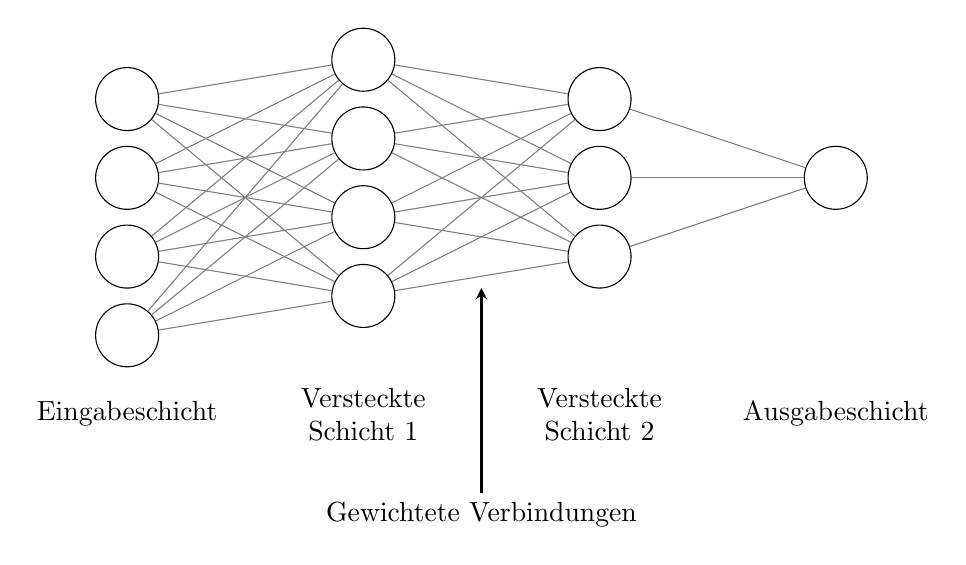
\begin{tikzpicture}[ neuron/.style={ circle, draw, minimum size=0.8cm }, >=stealth ] 
    % Eingabeschicht 
    \node[neuron] (i1) at (0,2) {}; 
    \node[neuron] (i2) at (0,1) {}; 
    \node[neuron] (i3) at (0,0) {}; 
    \node[neuron] (i4) at (0,-1) {}; 
    % Hidden Layer 1 
    \node[neuron] (h11) at (3,2.5) {}; 
    \node[neuron] (h12) at (3,1.5) {}; 
    \node[neuron] (h13) at (3,0.5) {}; 
    \node[neuron] (h14) at (3,-0.5) {}; 
    % Hidden Layer 2 
    \node[neuron] (h21) at (6,2) {}; 
    \node[neuron] (h22) at (6,1) {}; 
    \node[neuron] (h23) at (6,0) {}; 
    % Ausgabeschicht 
    \node[neuron] (o1) at (9,1) {}; 
    % Verbindungen Input -> Hidden 1 
    \foreach \i in {1,2,3,4} { 
      \foreach \h in {1,2,3,4} { 
        \draw[gray] (i\i) -- (h1\h); 
      } 
    } 
    % Verbindungen Hidden 1 -> Hidden 2 
    \foreach \h in {1,2,3,4} { 
      \foreach \k in {1,2,3} { 
        \draw[gray] (h1\h) -- (h2\k); 
      } 
    } 
    % Verbindungen Hidden 2 -> Output 
    \foreach \k in {1,2,3} { 
      \draw[gray] (h2\k) -- (o1); 
    } 
    % Beschriftungen 
    \node[align=center] at (0,-2) {Eingabeschicht}; 
    \node[align=center] at (3,-2) {Versteckte\\Schicht 1}; 
    \node[align=center] at (6,-2) {Versteckte\\Schicht 2}; 
    \node[align=center] at (9,-2) {Ausgabeschicht}; 
    % Pfeil für gewichtete Verbindungen 
    \draw[->, thick] (4.5,-3) -- (4.5,-0.4);
    \node[below] at (4.5,-3) {Gewichtete Verbindungen}; 
  \end{tikzpicture} 
  \caption{Schematischer Aufbau eines mehrschichtigen neuronalen Netzes} 
  \label{fig:neuronales_netz} 
\end{figure}


\subsection{Vektoren, Vektorraum, Embeddings und Embedding-Raum}

Vektoren sind geordnete Mengen von Zahlen, die in der Mathematik und Informatik verwendet werden, um Objekte im mehrdimensionalen Vektorraum darzustellen. 
In der Verarbeitung natürlicher Sprache werden Wörter, Sätze und Dokumente häufig in Vektoren überführt.
Ein anderes Wort für diese Vektoren ist Embeddings. Embeddings ermöglichen es, semantische Ähnlichkeiten zwischen Wörtern zu erfassen, indem ähnliche Wörter im mehrdimensionalen Embedding-Raum (vergleiche Abbildung \ref{fig:embedding3d}) nahe beieinander liegen.
Der Embedding-Raum ist der mehrdimensionale Raum, in dem diese Embeddings angeordnet sind. 
In diesem Raum repräsentieren die Positionen der Embeddings die semantischen Beziehungen zwischen den entsprechenden Wörtern. 
Jedes Wort wird dabei durch mehrere Zahlenwerte, die verschiedene Merkmale des Wortes repräsentieren, in einem Embedding dargestellt.
Die einzelnen Dimensionen eines Embeddings besitzen hier keine direkte, für Menschen verständliche Bedeutung.
Erst die Position der Embeddings im Raum ermöglicht es, semantische Ähnlichkeiten zwischen Wörtern zu erkennen \parencite{Mikolov2013}.

Ein Embedding kann dabei wie folgt veranschaulicht werden:

\[ \mathbf{e}_{\text{Katze}} = \begin{bmatrix} 0.82 \\ -0.15 \\ 0.47 \end{bmatrix} \]

Dieses Embedding repräsentiert das Wort „Katze“ im mehrdimensionalen Embedding-Raum, wobei jede Komponente des Vektors ein bestimmtes Merkmal oder eine Eigenschaft des Wortes „Katze“ kodiert.
Um die Funktionalität von Embeddings weiter zu verdeutlichen, sollen hier mehrere Embeddings für verschiedene Wörter exemplarisch betrachtet werden:

\[ 
\mathbf{e}_{\text{Katze}} 
= 
\begin{bmatrix} 
  0.82\\ 
  -0.15\\ 
  0.47 
\end{bmatrix}, 
\qquad 
\mathbf{e}_{\text{Hund}} 
= 
\begin{bmatrix} 
  0.79\\ 
  -0.12\\ 
  0.51 
\end{bmatrix}, 
\qquad 
\mathbf{e}_{\text{Auto}} 
= 
\begin{bmatrix} 
  -0.34\\ 
  0.88\\ 
  0.70 
\end{bmatrix} 
\]

Abbildung \ref{fig:embedding3d} zeigt die Position dieser Embeddings in einem vereinfachten dreidimensionalen Embedding-Raum. 
Da die Koordinaten der Wörter „Katze“ und „Hund“ sehr ähnlich sind, liegen ihre Positionen nahe beieinander. 
Das Embedding des Wortes „Auto“ unterscheidet sich dagegen stärker von „Katze“ oder „Hund“ und befindet sich deshalb weiter entfernt. 

\begin{figure}[ht] 
  \centering 
  \tdplotsetmaincoords{70}{115} 
  \begin{tikzpicture}[tdplot_main_coords, scale=3] 
    % Achsen 
    \draw[->] (-0.6,0,0) -- (1.1,0,0) node[right] {x}; 
    \draw[->] (0,-0.4,0) -- (0,1.1,0) node[left] {y}; 
    \draw[->] (0,0,-0.4) -- (0,0,0.8) node[above] {z}; 
    % Katze 
    \filldraw[blue] (0.82,-0.15,0.47) circle (1pt) node[above left] {Katze}; 
    % Hund 
    \filldraw[blue] (0.79,-0.12,0.51) circle (1pt) node[right] {Hund}; 
    % Auto 
    \filldraw[red] (-0.34,0.88,0.70) circle (1pt) node[left] {Auto}; 
  \end{tikzpicture} 
  \caption{Vereinfachte Darstellung der Beispiel-Embeddings im dreidimensionalen Embedding-Raum} 
  \label{fig:embedding3d} 
\end{figure}


\section {Modellansätze}

\subsection{Neural Language Models}

Neuronale Sprachmodelle (Neural Language Models, NLMs) sind spezielle neuronale Netze, die auf Textsammlungen, 
sogenannten Textkorpora, vortrainiert werden, um sprachliche Muster, semantische Zusammenhänge sowie Wissensrepräsentationen zu erlernen.
Hierzu werden Wörter, Sätze und Dokumente in Embeddings überführt, die als Eingabe für das neuronale Netz dienen \parencite{LeCun2015}.

\subsection{Large Language Models }

Large Language Models (LLMs) basieren auf neuronalen Sprachmodellen und erweitern diese durch eine enorme Anzahl an Parametern sowie tieferen Architekturen.
Sie bilden die Grundlage für generative KI-Systeme und ermöglichen die Bearbeitung von verschiedenen Aufgaben aus dem bereich der natürlichen Sprachverarbeitung.
Dazu zählen Textgenerierung, Textklassifikation, Frage-Antwort-Systeme sowie das liefern mehrer relevanter Ergebnisse zu einer Suchanfrage, dem sogenannten Information Retrieval \parencite{Zhao2023}.

Moderne LLMs bestehen typischerweise aus mehreren Milliarden Parametern. Während des Trainings werden hierbei diese Modellparameter wie in \autoref{subsec:modell} beschrieben auf Zusammenhänge gelernt. 
Diese Zusammenhänge beziehen sich hier auf die statistischen Beziehungen zwischen Wörtern, Sätzen und Dokumenten.
Dadurch können LLMs Aufgaben Lösen, auf die sie nicht explizit trainiert wurden, da die Antwort auf eine Eingabe aus dem erlernten Wissen abgeleitet werden kann. 
Hierbei spielt die Generalisierungsfähigkeit des Modells eine entscheidende Rolle. Anhand dieser Fähigkeit wird die Leistungsfähigkeit eines LLMs bei der Bearbeitung neuer, bisher unbekannter Aufgaben bewertet \parencite{Zhao2023}.

Die Architektur hinter einem LLM basiert auf dem Transformer-Modell. Dieses Modell nutzt sogenannte Attention-Mechanismen, um die statistischen Zusammenhänge zwischen einzelen Wörtern in einem Satz zu erfassen und zu gewichten \parencite{Vaswani2017}. 
Ein Beispiel hierfür ist folgender Satz: „Anna trinkt Kaffee am Morgen.“ Der Attention-Mechanismus bewertet die Bedeutung jedes Wortes im Zusammenhang mit den anderen Wörtern des Satzes. 
Dabei erkennt das Modell, dass die Wörter „Anna“, „trinkt“ und „Kaffee“ stärker miteinander in Beziehung stehen als häufig vorkommende Wörter wie „am“ oder „der“. 

\subsection{Fine-Tuning}

Large Language Models werden auf allgemeine Textkorpora vortrainiert, um ein umfangreiches sprachliches und sachliches Wissen zu erwerben.
Dies führt dazu, dass das Modell ein breites Wissen über Sprach und Sachverhalte erwirbt, aber möglicherweise nicht auf spezifische Aufgaben oder einzelnen Fachbereiche spezialisiert ist.
Um ein LLM auf spezifische Aufgaben oder Fachbereiche anzupassen, wird häufig das sogenannte Fine-Tuning eingesetzt. 
Hierbei wird das vortrainierte LLM mit Informationen zu der spezifischen Aufgabe oder Fachbereichs weiter trainiert, 
um damit die Leistungsfähigkeit an die Anforderrungen des jeweiligen Einsatzbereichs anzupassen \parencite{Wei2022,Zhang2023InstructionTuning}.

Das Grundprinzip des Fine-Tunings ist es, dass ein vortrainiertes LLM nicht vollständig neu trainiert werden muss, 
sondern das vorhanden Wissen als Ausgangspunkt genutzt werden kann und mit Daten aus dem spezifischen Fachbereich weiter trainiert wird.
Dadurch ist es möglich, deutliche bessere Ergebnisse zu erzielen, als bei einem kompletten Neutraining eines neuronalen Sprachmodells
Dadurch ist der Trainigsaufwand im Vergleich zu einem vollständigen Neutraining deutlich geringer.\parencite{Wei2022}.

Um dies am obrigen Beispiel zu verdeutlichen: Angenommen, das LLM soll zusätzlich Informationen über die Vorlieben von Anna beim Kaffeetrinken lernen. 
Durch Fine-Tuning mit entsprechenden Daten kann das Modell die Aufmerksamkeit gezielt auf relevante Zusammenhänge lenken, wie zum Beispiel die Präferenz von Anna für bestimmte Kaffeesorten oder Zubereitungsarten.
Dabei wird dann der Attention-Mechanismus des Modells gezielt auf die neuen relevanten Informationen für Annas Kaffeetrinken ausgerichtet.


\subsection{Sentence Transformers}

Bei Sentence Transformers handelt es sich um neuronale Sprachmodelle, die vollständige Sätze oder Dokumente in Embeddings, überführen.
Das Ziel eines Sentence Transformers ist es, semantisch ähnliche Texte im Embedding-Raum nahe beieinander zu platzieren, während semantisch unterschiedliche Texte weiter voneinander entfernt liegen.
Sentence Transformers werden häufig für Aufgaben wie semantische Suche oder Empfehlungssysteme eingesetzt.
Anstatt ausschließlich identische Schlüsselwörter zu suchen, ermöglichen sie die Identifikation inhaltlich ähnlicher Dokumente auch dann, wenn unterschiedliche Formulierungen verwendet werden \parencite{Reimers2019SBERT}.

\begin{figure}[ht] 
  \centering 
  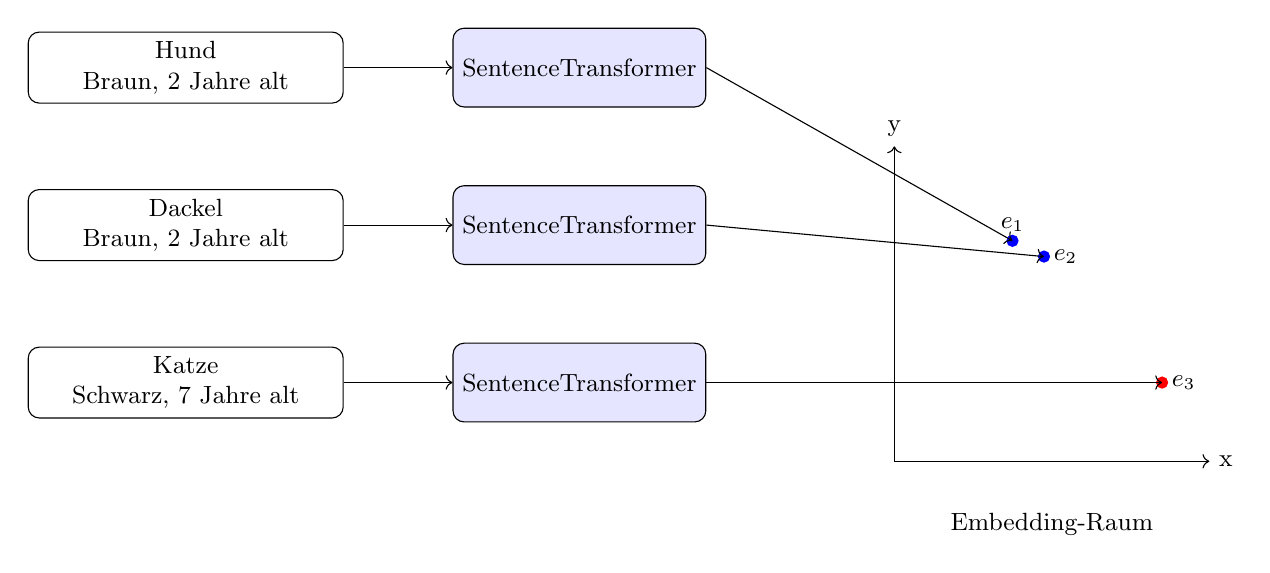
\begin{tikzpicture}[ 
    node distance=1.8cm, every node/.style={font=\small}, 
    textnode/.style=
    { draw, rounded corners, align=center, minimum width=4.0cm, minimum height=0.9cm }, 
    model/.style=
    { draw, fill=blue!10, rounded corners, minimum width=2.5cm, minimum height=1cm } ] 
    % Eingabetexte 
    \node[textnode] (t1) at (0,2) 
    {Hund\\Braun, 2 Jahre alt}; 
    \node[textnode] (t2) at (0,0) 
    {Dackel\\Braun, 2 Jahre alt}; 
    \node[textnode] (t3) at (0,-2) 
    {Katze\\Schwarz, 7 Jahre alt}; 
    % Sentence Transformer 
    \node[model] (m1) at (5,2) 
    {Sentence\\Transformer}; 
    \node[model] (m2) at (5,0) 
    {Sentence\\Transformer}; 
    \node[model] (m3) at (5,-2) 
    {Sentence\\Transformer}; 
    % Pfeile zum Modell 
    \draw[->] (t1) -- (m1); 
    \draw[->] (t2) -- (m2); 
    \draw[->] (t3) -- (m3); 
    % Embedding-Raum 
    \draw[->] (9,-3) -- (13,-3) node[right] {x}; 
    \draw[->] (9,-3) -- (9,1) node[above] {y}; 
    \node at (11,-3.8) {Embedding-Raum}; 
    % Punkte 
    \filldraw[blue] (10.5,-0.2) circle (2pt); 
    \node[above] at (10.5,-0.2) {$e_1$}; 
    \filldraw[blue] (10.9,-0.4) circle (2pt); 
    \node[right] at (10.9,-0.4) {$e_2$}; 
    \filldraw[red] (12.4,-2.0) circle (2pt); 
    \node[right] at (12.4,-2.0) {$e_3$}; 
    % Verbindungslinien 
    \draw[->] (m1.east) -- (10.5,-0.2); 
    \draw[->] (m2.east) -- (10.9,-0.4); 
    \draw[->] (m3.east) -- (12.4,-2.0); 
    \end{tikzpicture} 
    \caption{Prinzipielle Funktionsweise eines Sentence Transformers. Semantisch ähnliche Texte werden auf nahe beieinanderliegende Embeddings abgebildet, während inhaltlich unterschiedliche Texte größere Abstände im Embedding-Raum aufweisen.} 
    \label{fig:sentence_transformer} 
\end{figure}


\subsection{Embedding-Modelle}

\subsection{Triplet Loss}

\subsection{Learning-to-Rank}

Learning-to-Rank (LTR) bezeichnet eine Klasse von maschinellen Lernverfahren, die das Ziel besitzen, die Reihenfolge in einer Ergebnisliste zu optimieren \parencite{liu2009learning}.
Im Gegensatz zu klassischen Klassifikations- oder Regressionsansätzen bewertet Learning-to-Rank keine einzelnen Objekte isoliert, sondern die relative Relevanz dieser Objekte in einer Kandidatenmenge.
Die Aufgabe eines Rankingmodells besteht darin, dass für eine Anfrage die relevanten Dokumente anhand ihrer Merkmale bewertet werden und anschließend in eine Rangliste überführt werden.

\subsection{LambdaRank}

\section{Validierungsansätze}

\subsection{Recall@k} 

Recall@k gehört zu den grundlegenden Bewertungsmetriken des Information Retrievals und beschreibt den Anteil der Anfragen, bei denen mindestens ein relevantes Ergebnis innerhalb der ersten $k$ Rangpositionen gefunden wird \parencite{manning2008ir}. 
Diese Metrik berechnet sich wie folgt: 

\begin{align} 
  Recall@k = \frac{ \# \text{Anfragen mit relevantem Ergebnis in Top-}k }{ \# \text{Anfragen} } 
\end{align} 

mit 

\begin{description} 
    \item[$k$]: Anzahl der betrachteten Rangpositionen 
    \item[$\text{Anfragen mit relevantem Ergebnis in Top-}k$]: Anzahl erfolgreicher Anfragen 
    \item[$\text{Anfragen}$]: Gesamtzahl aller Anfragen 
\end{description} 

Der Wertebereich liegt zwischen 0 und 1. Ein Wert von 1 bedeutet, dass sich für jede Anfrage mindestens ein relevantes Ergebnis innerhalb der Top-$k$ Positionen der Rangliste befindet. 
In Ranking- und Empfehlungssystemen wird Recall@k häufig verwendet, um die praktische Verwendung eines Systems beurteilen zu können.
Der Anwender betrachtet dabei in der Regel nur die ersten Ergebnisse einer Rangliste \parencite{manning2008ir}.

\subsection{Mean Reciprocal Rank} 

Der Mean Reciprocal Rank (MRR) zählt neben Recall@k zu etablierten Bewertungsmetriken des Information Retrievals und wird sowohl in klassischen Suchsystemen als auch in modernen Rankingverfahren eingesetzt \parencite{voorhees1999mrr,zhu2024llmirsurvey}. 
Mit dieser Kennzahl wird die Position des ersten relevanten Ergebnisses innerhalb einer Rangliste bewertet.

Die Berechnung ergibt sich wie folgt:  

\begin{align} 
  MRR= \frac{1}{N} \sum_{i=1}^{N} \frac{1}{rank_i} 
\end{align} 

mit 

\begin{description} 
    \item[$N$] Anzahl der ausgewerteten Anfragen 
    \item[$rank_i$] Rangposition des ersten relevanten Ergebnisses für Anfrage $i$ 
\end{description} 

Der Wertebereich liegt zwischen 0 und 1. Ein hoher Wert zeigt an, dass ein relevantes Ergebnis bereits an einer der vorderen Positionen einer Rangliste erscheint. 
Da frühe Treffer stärker gewichtet werden als spätere Treffer, eignet sich die Kennzahl besonders zur Bewertung der schnellen Auffindbarkeit relevanter Ergebnisse.

\subsection{Normalized Discounted Cumulative Gain} 

Der Discounted Cumulative Gain (DCG) wurde von Järvelin und Kekäläinen zur Bewertung verschiedener Relevanzstufen von Suchergebnissen eingeführt und zählt zu den wichtigsten Bewertungsmetriken für Ranking- und Suchsysteme \parencite{jarvelin2002dcg}. 
Die Kennzahl berücksichtigt sowohl die Relevanz eines Ergebnisses als auch die Position innerhalb der Rangliste. Relevante Ergebnisse auf frühen Rangpositionen leisten dadurch einen höheren Beitrag zur Gesamtbewertung. 

Die Berechnung des DCG erfolgt über 

\begin{align} 
  DCG@k = \sum_{i=1}^{k} \frac{2^{rel_i}-1} {\log_2(i+1)} 
\end{align} 

mit 

\begin{description} 
  \item[$k$] Anzahl der betrachteten Rangpositionen 
  \item[$i$] Rangposition innerhalb der Rangliste 
  \item[$rel_i$] Relevanzwert des Ergebnisses auf Rangposition $i$ 
\end{description} 

Um eine bessere Vergleichbarkeit zu schaffen, findet eine Normierung auf die ideale Rangliste statt. Hieraus ergibt sich der Normalized Discounted Cumulative Gain (nDCG): 

\begin{align} 
nDCG@k= \frac{DCG@k} {IDCG@k} 
\end{align} 
mit 
\begin{description} 
  \item[$DCG@k$] DCG-Wert der betrachteten Rangliste 
  \item[$IDCG@k$] \textit{Ideal Discounted Cumulative Gain}, also der höchstmögliche DCG-Wert, der bei einer idealen Sortierung der Kandidaten nach absteigender Relevanz erreicht würde 
\end{description} 

Der Wertebereich liegt zwischen 0 und 1. Ein Wert von 1 entspricht der optimal möglichen Rangfolge.

\subsection{Hierarchische Bewertungsmetriken} 

Nicht jede fachliche Fehlentscheidung hat in technischen Empfehlungssystemen dieselbe Bedeutung.
Ein Ergebnis kann beispielsweise einer technisch verwandten Produkt- oder Makrofamilie angehören, aber trotz fehlender exakter Übereinstimmung für den Anwender weiterhin von Interesse sein. 
Zur Berücksichtigung solcher Beziehungen werden hierarchische Bewertungsmetriken eingesetzt. 

Diese basieren typischerweise auf dem Discounted Cumulative Gain \parencite{jarvelin2002dcg} und verwenden unterschiedliche Relevanzen in abgestufter Reihenfolge. 

Eine mögliche Relevanzfunktion lautet: 

\begin{align} 
rel = 
\begin{cases} 3,& \text{exakte Übereinstimmung}\\ 2,& \text{gleiche Familie}\\ 0,& \text{keine fachliche Beziehung} 
\end{cases} \end{align} 

Dadurch wird eine Rangliste bevorzugt, welche fachlich ähnliche Kandidaten auf höheren Positionen platziert. 
Hierarchische Bewertungsmetriken eignen sich insbesondere für industrielle Empfehlungssysteme, bei denen zwischen exakter Übereinstimmung und fachlicher Nähe unterschieden werden muss.

\section{Handlungsbedarf}
\chapter{Zielsetzung und Vorgehensweise} 

\section{Zielsetzung}

Das Projektziel ist die Entwicklung eines Systems, welches automatisiert EPLAN-Artikel \parencite{EPLANArtikelverwaltung} zu EPLAN-Fenstermakros \parencite{EPLAN-Makros} zuordnet.
Für einen vorhanden technischen EPLAN-Artikel \parencite{EPLANArtikelverwaltung} soll anhand einer technischen Anfrage (zum Beispiel in Form eines Datenblatts) das fachlich passendste EPLAN-Fenstermakro \parencite{EPLAN-Makros} identifiziert werden.


Diese Problemstellung kann als Rankingaufgabe formuliert werden, bei der für jede Anfrage eine Menge bekannter EPLAN-Fenstermakros \parencite{EPLAN-Makros} vorliegt. Dabei sind alle Kandidaten dieser Menge potenzielle Ergebnisse für den 1. Rang.
Das System soll die Eigenschaften eines gegebenen EPLAN-Artikels \parencite{EPLANArtikelverwaltung} analysieren und diese mit allen verfügbaren Makro-Kandidatenprofilen vergleichen. Anschließend sollen die Kandidaten entsprechend ihrer Relevanz geordnet werden.
Ziel dabei ist es, dass das passendste EPLAN-Fenstermakro \parencite{EPLAN-Makros} möglichst auf Rang 1 erscheint. Die weniger ähnlichen Kandidaten sollen entsprechend der Bewertung hierarchisch auf den nachfolgenden Rängen einsortiert werden.


Im Gegensatz zu Klassifikationsaufgaben liegt der Fokus dieses Systems nicht direkt auf der Bestimmung einer einzelnen Klasse oder Produktfamilie. Vielmehr geht es darum eine möglichst präzise Variantenauflösung zu erreichen.
Dafür sollen die technischen Eigenschaften und Merkmale aus einer Anfrage systematisch erfasst und mit den Eigenschaften der EPLAN-Artikel \parencite{EPLANArtikelverwaltung} abgeglichen werden.


Die Herausforderung besteht darin, dass sich viele Produkte lediglich in einzelnen technischen Eigenschaften und Konfigurationsmerkmalen unterscheiden. Geringe Abweichungen können deshalb zu unterschiedlichen Makrozuordnungen führen.
Das System muss daher in der Lage sein allgemeine technischen Zusammenhänge als auch merkmalspezifische Unterschiede zwischen ähnlichen Varianten zu erkennen.


Zur Lösung dieses Problems wird ein Learning-to-Rank-System entwickelt, welches strukturierte technische sowie lexikalische Merkmale aus Artikeldaten kombiniert, um die Relevanz von potenziellen EPLAN-Fenstermakros \parencite{EPLAN-Makros} zu bewerten. 
Das Modell erzeugt für jeden verfügbaren Makrokandidaten eine Relevanzbewertung und erstellt daraus eine Rangliste möglicher Empfehlungen. Ziel ist es, das korrekte Zielmakro möglichst auf den vorderen Rangpositionen, idealerweise auf Rang 1, zu platzieren.

\section{Methodisches Vorgehen}

Das methodische Vorgehen orientiert sich an der \textit{Design Science Research Methodology} (DSRM) nach Peffers et al. \citeyearpar{peffers2007dsrm}. 
Die DSRM beschreibt einen strukturierten Forschungsprozess zur Entwicklung und Evaluation technischer Artefakte und eignet sich insbesondere für die Entwicklung von IT-Systemen.
Das Ziel der Methodik besteht darin, eine konkrete Problemstellung systematisch zu analysieren, ein geeignetes Artefakt zu entwickeln und den Nutzen durch eine Evaluation nachzuweisen. 

Der von Peffers et al. beschriebene Forschungsprozess umfasst die folgenden Schritte: 

\begin{enumerate} 
    \item Problemidentifikation und Motivation 
    \item Definition der Lösungsziele 
    \item Design und Entwicklung des Artefakts 
    \item Demonstration der entwickelten Lösung 
    \item Evaluation des Artefakts 
    \item Kommunikation der Ergebnisse 
\end{enumerate} 

In dieser Arbeit bildet die DSRM den übergeordneten Rahmen. Die iterative Entwicklung des Ranking-Systems erfolgt innerhalb der Design-, Entwicklungs- und Evaluationsphase durch wiederkehrende Entwicklungszyklen. 

\section{Iterativer Entwicklungsprozess} 

Zur Entwicklung des Artefakts wird die Design-Science-Methodik durch die Prinzipien des \textit{Action Design Research} (ADR) nach Sein et al. verwendet \citeyearpar{sein2011adr}. 
ADR verbindet dabei die Entwicklung eines Artefakts mit der fortlaufenden Anwendung, Evaluation und Verbesserung. 
Während die DSRM den strukturellen Prozess beschreibt, liefert ADR den Entwicklungszyklus zur kontinuierlichen Verbesserung des Systems. 

Der iterative Entwicklungsprozess besteht dabei aus den folgenden Schritten: 

\begin{enumerate} 
    \item Analyse des aktuellen Zustands und Identifikation von Verbesserungspotentialen 
    \item Recherche wissenschaftlicher und technischer Lösungen
    \item Konzeption neuer Komponenten, Merkmale oder Optimierungen
    \item Implementierung und Anpassung der entwickelten Ansätze 
    \item Durchführung von Tests und Validierungen 
    \item Evaluation anhand definierter Qualitätsmetriken 
    \item Interpretation der Ergebnisse 
    \item Ableitung weiterer Verbesserungen
\end{enumerate} 

Die Ergebnisse einer Iteration bilden jeweils die Grundlage für die nachfolgenden Iterationen. Auf diese Weise entsteht ein kontinuierlicher Verbesserungsprozess, in dem Forschung, Entwicklung, Evaluation und Optimierung miteinander verzahnt sind. 
Die Kombination aus DSRM und ADR ermöglicht somit auf der einen Seite einen strukturierten Forschungsprozess und auf der anderen Seite eine iterative Verbesserung des entwickelten Ranking-Systems. 
Abbildung \ref{fig:dsrm_adr_verzahnung} veranschaulicht diese Verzahnung der beiden Methodiken.

Die theoretischen Grundlagen der verwendeten Bewertungsmetriken wurden bereits in Kapitel \ref{chap:stand_der_technik} vorgestellt. 
Die Anwendung dieser Metriken zur Bewertung des entwickelten Systems erfolgt in Kapitel \ref{chap:evaluierungskonzept}.
Eine Darstellung der finalen Systemarchitektur und der vollständigen Pipeline befindet sich ebenfalls in diesem Kapitel.


\begin{figure}[tbp]
    \centering
    \resizebox{\textwidth}{!}{%
    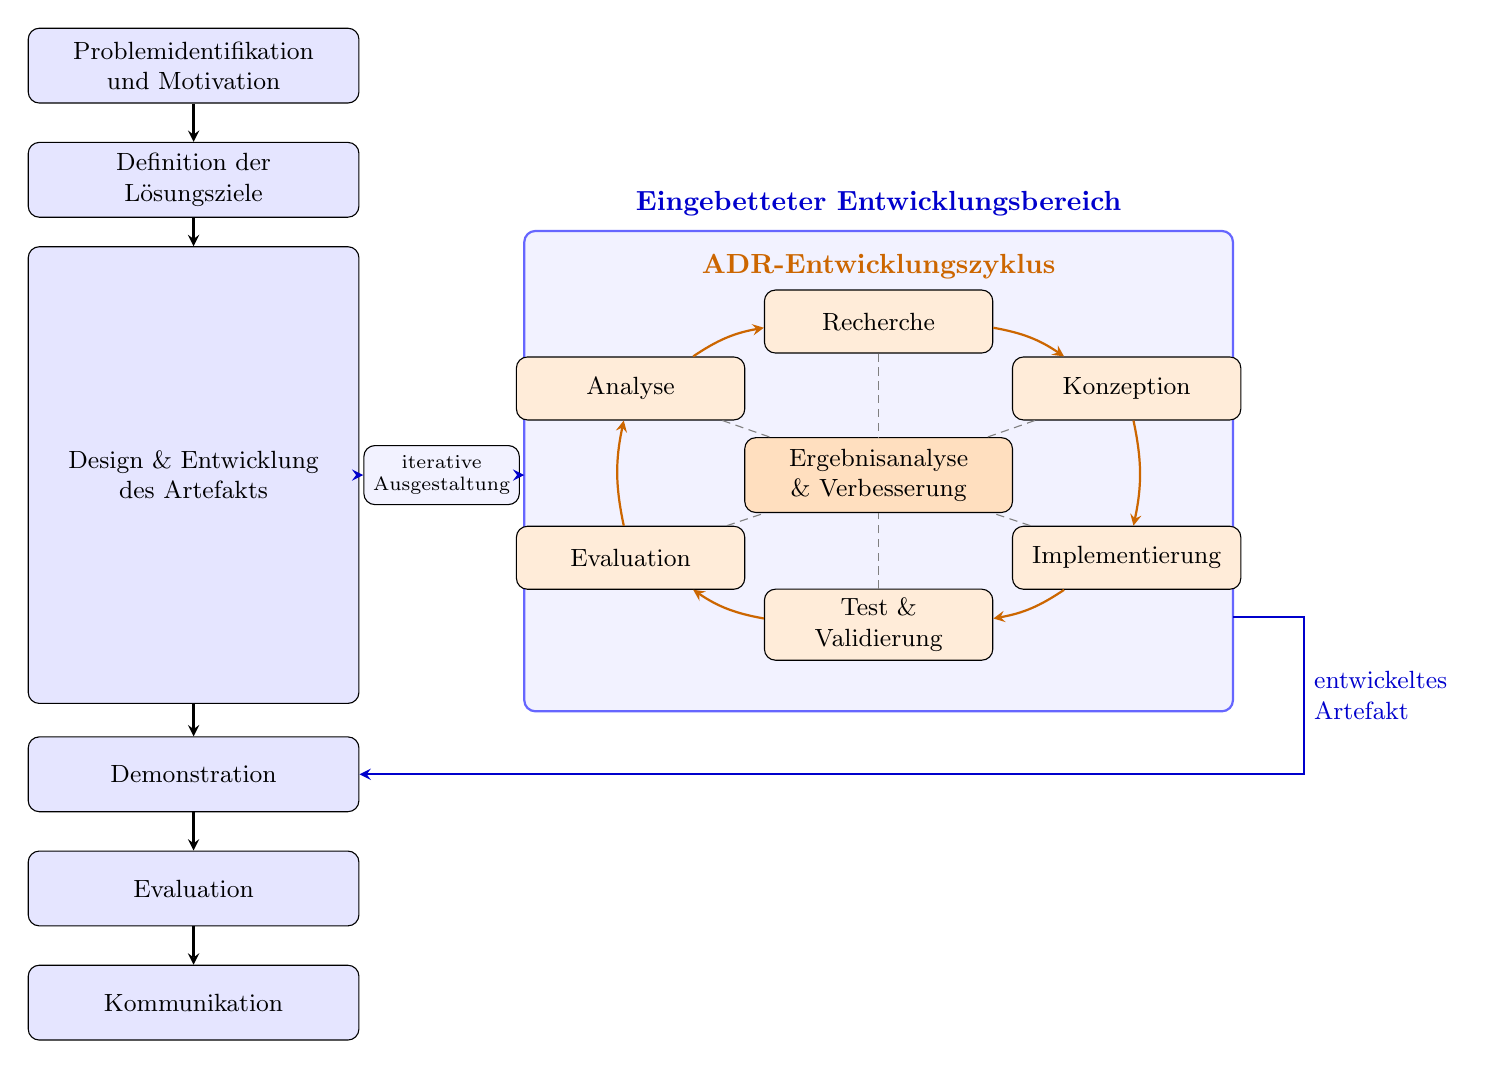
\begin{tikzpicture}[
        >=stealth,
        font=\small,
        dsrm/.style={draw, rounded corners, fill=blue!10, minimum width=4.2cm, minimum height=0.95cm, align=center},
        adr/.style={draw, rounded corners, fill=orange!15, minimum width=2.9cm, minimum height=0.8cm, align=center},
        analysis/.style={draw, rounded corners, fill=orange!25, minimum width=3.4cm, minimum height=0.95cm, align=center},
        bridge/.style={draw, rounded corners, fill=blue!5, minimum width=1.8cm, minimum height=0.75cm, align=center, font=\scriptsize},
        flow/.style={->, thick},
        cycle/.style={->, thick, orange!80!black},
        relation/.style={densely dashed, gray},
        artifact/.style={->, thick, blue!80!black}
    ]

        \node[dsrm] (problem) at (0, 0) {Problemidentifikation\\und Motivation};
        \node[dsrm] (goals) at (0, -1.45) {Definition der\\Lösungsziele};
        \node[dsrm, minimum height=5.8cm] (designphase) at (0, -5.2) {Design \& Entwicklung\\des Artefakts};
        \node[dsrm] (demo) at (0, -9.0) {Demonstration};
        \node[dsrm] (eval) at (0, -10.45) {Evaluation};
        \node[dsrm] (comm) at (0, -11.9) {Kommunikation};

        \draw[flow] (problem) -- (goals);
        \draw[flow] (goals) -- (designphase);
        \draw[flow] (designphase) -- (demo);
        \draw[flow] (demo) -- (eval);
        \draw[flow] (eval) -- (comm);

        \draw[blue!60, thick, rounded corners, fill=blue!5]
            (4.2, -2.1) rectangle (13.2, -8.2);
        \node[font=\bfseries, text=blue!80!black, align=center] at (8.7, -1.75)
            {Eingebetteter Entwicklungsbereich};

        \node[font=\bfseries, text=orange!80!black] at (8.7, -2.55)
            {ADR-Entwicklungszyklus};
        \node[adr] (analyse) at (5.55, -4.1) {Analyse};
        \node[adr] (recherche) at (8.7, -3.25) {Recherche};
        \node[adr] (konzeption) at (11.85, -4.1) {Konzeption};
        \node[adr] (implement) at (11.85, -6.25) {Implementierung};
        \node[adr] (test) at (8.7, -7.1) {Test \&\\Validierung};
        \node[adr] (adreview) at (5.55, -6.25) {Evaluation};
        \node[analysis] (improve) at (8.7, -5.2) {Ergebnisanalyse\\\& Verbesserung};

        \draw[cycle] (analyse) to[bend left=12] (recherche);
        \draw[cycle] (recherche) to[bend left=12] (konzeption);
        \draw[cycle] (konzeption) to[bend left=12] (implement);
        \draw[cycle] (implement) to[bend left=12] (test);
        \draw[cycle] (test) to[bend left=12] (adreview);
        \draw[cycle] (adreview) to[bend left=12] (analyse);

        \foreach \n in {analyse,recherche,konzeption,implement,test,adreview} {
            \draw[relation] (\n) -- (improve);
        }

        \node[bridge] (iteration) at (3.15, -5.2) {iterative\\Ausgestaltung};
        \draw[artifact] (designphase.east) -- (iteration.west);
        \draw[artifact] (iteration.east) -- (4.2, -5.2);
        \draw[artifact] (13.2, -7.0) -- ++(0.9, 0) |- node[pos=0.25, right, align=left] {entwickeltes\\Artefakt} (demo.east);

    \end{tikzpicture}%
    }

    \caption{Verzahnung von DSRM und ADR. Die DSRM bildet den übergeordneten Forschungsrahmen, während ADR als iterativer Entwicklungszyklus innerhalb der Phase \glqq Design \& Entwicklung des Artefakts\grqq\ eingesetzt wird.}
    \label{fig:dsrm_adr_verzahnung}
\end{figure}












\chapter{Architekturübersicht}
\label{chap:architektur}

\section{Gesamtarchitektur}

Die entwickelte Lösung basiert auf einer mehrstufigen Architektur, die aus Retrieval-, Feature-Engineering- und Ranking-Komponenten besteht. 
Im Gegensatz zu klassischen Suchsystemen, bei denen auf eine Anfrage direkte Ergebnisse gerankt werden, wird in diesem System ein anderer Ansatz verwendet.
Dabei werden mehrere Retrievalsignale erzeugt, die im Anschluss zusammen mit technischen Merkmalen als Eingabe für das Learning-to-Rank-Modell verwendet werden.

Die einzelnen Schritte der Pipeline reichen von der Datenaufbereitung, über die Kandidatenbildung bis hin zum modellbasierten Ranking.

Abbildung \ref{fig:architektur} zeigt die implementierte End-to-End-Pipeline des Systems.

\usetikzlibrary{positioning, arrows.meta}

\begin{figure}[htbp]
    \centering
    \resizebox{!}{0.68\textheight}{%
    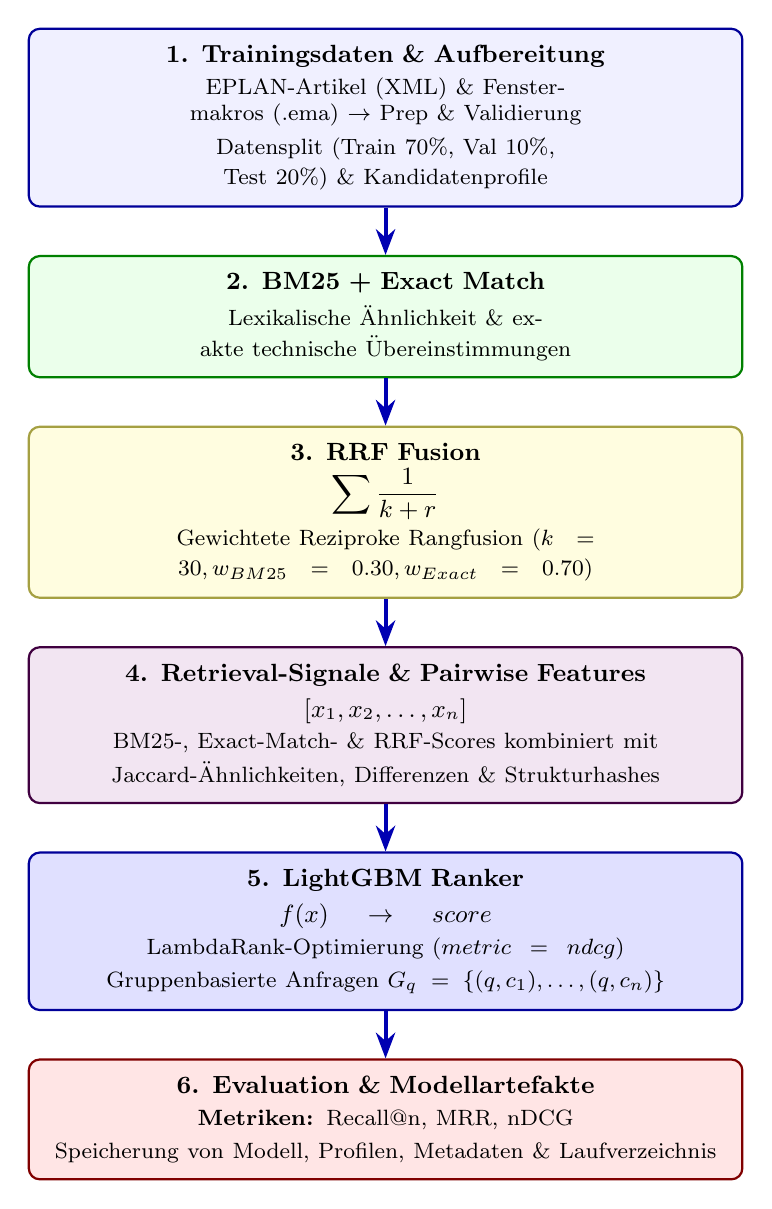
\begin{tikzpicture}[
        >=Stealth,
        font=\small,
        databox/.style={draw=blue!60!black, thick, rounded corners=4pt, fill=blue!6, text width=8.5cm, minimum height=1.2cm, align=center, inner ysep=6pt, inner xsep=8pt},
        retbox/.style={draw=green!50!black, thick, rounded corners=4pt, fill=green!8, text width=8.5cm, minimum height=1.1cm, align=center, inner ysep=6pt, inner xsep=8pt},
        fusionbox/.style={draw=yellow!60!black, thick, rounded corners=4pt, fill=yellow!12, text width=8.5cm, minimum height=1.2cm, align=center, inner ysep=6pt, inner xsep=8pt},
        featurebox/.style={draw=violet!50!black, thick, rounded corners=4pt, fill=violet!10, text width=8.5cm, minimum height=1.3cm, align=center, inner ysep=6pt, inner xsep=8pt},
        modelbox/.style={draw=blue!60!black, thick, rounded corners=4pt, fill=blue!12, text width=8.5cm, minimum height=1.3cm, align=center, inner ysep=6pt, inner xsep=8pt},
        evalbox/.style={draw=red!50!black, thick, rounded corners=4pt, fill=red!10, text width=8.5cm, minimum height=1.2cm, align=center, inner ysep=6pt, inner xsep=8pt},
        flow/.style={->, >=Stealth, line width=1.4pt, blue!70!black}
    ]
        % Block 1: Trainingsdaten
        \node[databox] (data) {
            \textbf{1. Trainingsdaten \& Aufbereitung}\\[2pt]
            \footnotesize EPLAN-Artikel (XML) \& Fenstermakros (.ema) $\rightarrow$ Prep \& Validierung\\[1pt]
            Datensplit (Train 70\%, Val 10\%, Test 20\%) \& Kandidatenprofile
        };

        % Block 2: BM25 + Exact Match
        \node[retbox, below=0.6cm of data] (retrieval) {
            \textbf{2. BM25 + Exact Match}\\[2pt]
            \footnotesize Lexikalische Ähnlichkeit \& exakte technische Übereinstimmungen
        };

        % Block 3: RRF Fusion
        \node[fusionbox, below=0.6cm of retrieval] (rrf) {
            \textbf{3. RRF Fusion}\\[2pt]
            \small $\displaystyle \sum \frac{1}{k + r}$\\[2pt]
            \footnotesize Gewichtete Reziproke Rangfusion ($k=30, w_{\text{BM25}}=0.30, w_{\text{Exact}}=0.70$)
        };

        % Block 4: Retrieval-Signale als Features
        \node[featurebox, below=0.6cm of rrf] (features) {
            \textbf{4. Retrieval-Signale \& Pairwise Features}\\[2pt]
            \small $[x_1, x_2, \dots, x_n]$\\[2pt]
            \footnotesize BM25-, Exact-Match- \& RRF-Scores kombiniert mit\\[1pt]
            Jaccard-Ähnlichkeiten, Differenzen \& Strukturhashes
        };

        % Block 5: LightGBM Ranker
        \node[modelbox, below=0.6cm of features] (ranker) {
            \textbf{5. LightGBM Ranker}\\[2pt]
            \small $f(x) \rightarrow \text{score}$\\[2pt]
            \footnotesize LambdaRank-Optimierung ($\text{metric}=\text{ndcg}$)\\[1pt]
            Gruppenbasierte Anfragen $G_q = \{(q,c_1),\dots,(q,c_n)\}$
        };

        % Block 6: Evaluation
        \node[evalbox, below=0.6cm of ranker] (eval) {
            \textbf{6. Evaluation \& Modellartefakte}\\[2pt]
            \footnotesize \textbf{Metriken:} Recall@n, MRR, nDCG\\[1pt]
            Speicherung von Modell, Profilen, Metadaten \& Laufverzeichnis
        };

        % Verbindungen (Ablaufkette von 1 -> 2 -> 3 -> 4 -> 5 -> 6)
        \draw[flow] (data.south) -- (retrieval.north);
        \draw[flow] (retrieval.south) -- (rrf.north);
        \draw[flow] (rrf.south) -- (features.north);
        \draw[flow] (features.south) -- (ranker.north);
        \draw[flow] (ranker.south) -- (eval.north);
    \end{tikzpicture}%
    }
    \caption{Architektur der Trainings- und Rankingpipeline.}
    \label{fig:architektur}
\end{figure}


Die Orchestrierung aller Verarbeitungsschritte erfolgt zentral über die Trainingspipeline \cite{srcPipeline}.
\chapter{Analyse der Datenstrukturen und Ableitung eines Trainingsformats}
\label{chap:analyse_der_datenstrukturen}

\section{Analyse der Ausgangsdaten}

Die Datengrundlage für das entwickelte System bilden EPLAN-Artikel \parencite{EPLANArtikelverwaltung} und EPLAN-Fenstermakros \parencite{EPLAN-Makros}. Diese liegen in Form von strukturierten XML-Dateien und .ema-Dateien, einem XML-ähnlichen Format, vor \parencite{srcStep911}.
Um diese Daten für ein Learning-to-Rank-System nutzbar zu machen, müssen diese zunächst aufbereitet und in ein maschinenverständliches Format überführt werden.

Das Ziel der Datenaufbereitung besteht darin, alle technisch wichtigen Informationen der EPLAN-Artikel \parencite{EPLANArtikelverwaltung} sowie die strukturellen Merkmale der EPLAN-Fenstermakros \parencite{EPLAN-Makros} zu extrahieren. Auf dieser Grundlage kann die Eignung eines EPLAN-Artikels \parencite{EPLANArtikelverwaltung} für ein EPLAN-Fenstermakro \parencite{EPLAN-Makros} bewertet werden. 
Die Umsetzung dieser Datenaufbereitung erfolgt innerhalb der entwickelten Trainings- und Rankingpipeline \parencite{srcStep911,srcPipeline}.

\section{Analyse der Makrostrukturen}

Die Analyse der Makrostrukturen der EPLAN-Fenstermakros \parencite{EPLAN-Makros} konzentriert sich auf die enthaltenen Funktions- und Strukturmerkmale, welche die Grundstruktur und Funktionalität der Makros bestimmen \parencite{srcStep911}.
Tabelle \ref{tab:makrostrukturmerkmale} fasst die analysierten Merkmalsgruppen, die jeweils extrahierten Informationen und deren Bedeutung zusammen.

\begin{table}[tbp]
    \centering
    \setlength{\tabcolsep}{4pt}
    \renewcommand{\arraystretch}{1.08}
    \caption{Analysierte Merkmalsgruppen der EPLAN-Fenstermakros}
    \label{tab:makrostrukturmerkmale}
    \begin{tabularx}{\textwidth}{>{\raggedright\arraybackslash}p{4.0cm} >{\raggedright\arraybackslash}X}
        \toprule
        \textbf{Merkmalsgruppe} & \textbf{Extrahierte Merkmale und Bedeutung} \\
        \midrule
        Function-Template-\newline Struktur &
        \textbf{Merkmale:} Function-Template-Kategorien, Function-Template-Gruppen, Function-Template-IDs, Function-Template-Sequenzen, Struktur-Hashes, Sequenz-Hashes.\newline
        \textbf{Bedeutung:} Function-Templates sind grundlegende Bausteine, welche die Funktionalität und Logik der EPLAN-Fenstermakros \parencite{EPLAN-Makros} im EPLAN-System \parencite{eplan2026} bestimmen. Die Merkmale beschreiben die funktionale Struktur und ermöglichen die Identifikation ähnlicher oder identischer Makrostrukturen. \\
        \addlinespace
        Anschluss- und\newline Signalstruktur &
        \textbf{Merkmale:} Anzahl der Anschlüsse, Anschlussrollen, Anschlussarten, Signalanzahlen, Kanalzahlen, I/O-Schemata, Klemmeninformationen.\newline
        \textbf{Bedeutung:} Beschreibt die technische Funktion sowie die Anschlusslogik eines EPLAN-Fenstermakros \parencite{EPLAN-Makros}. \\
        \addlinespace
        Geräteeigenschaften &
        \textbf{Merkmale:} Bus-Systeme, Steckersysteme, Safety-Eigenschaften, LED-Eigenschaften, Leistungsmerkmale, Kommunikationsinformationen.\newline
        \textbf{Bedeutung:} Ordnet Makros technisch im Maschinen- und Anlagenbau-Kontext ein. \\
        \addlinespace
        Varianten-\newline informationen &
        \textbf{Merkmale:} Variantenkennungen, Baugruppeninformationen, Konfigurationsmerkmale, produktspezifische Strukturinformationen.\newline
        \textbf{Bedeutung:} Unterstützt die Auflösung fachlich ähnlicher Varianten, die sich nur durch einzelne technische Eigenschaften oder Konfigurationsmerkmale unterscheiden. \\
        \bottomrule
    \end{tabularx}
\end{table}

Die Makrostrukturmerkmale werden beim Aufbau der Makrokandidatenprofile gespeichert. In der regulären Query-Kandidat-Feature-Berechnung werden diese jedoch nicht direkt mit einer unbekannten Artikelanfrage verglichen, da deren Zielmakrostruktur zur Anfragezeit nicht verfügbar ist.

\section{Aufbereitung der Artikeldaten}

Neben den vorhandenen EPLAN-Fenstermakros \parencite{EPLAN-Makros} werden auch die EPLAN-Artikeldaten \parencite{EPLANArtikelverwaltung} aufbereitet und analysiert \parencite{srcStep911}.
Die verwendeten Merkmalsgruppen sind in Tabelle \ref{tab:artikelmerkmale} zusammengefasst.

\begin{table}[tbp]
    \centering
    \setlength{\tabcolsep}{4pt}
    \renewcommand{\arraystretch}{1.08}
    \caption{Aufbereitete Merkmalsgruppen der EPLAN-Artikeldaten}
    \label{tab:artikelmerkmale}
    \begin{tabularx}{\textwidth}{>{\raggedright\arraybackslash}p{4.8cm} >{\raggedright\arraybackslash}X}
        \toprule
        \textbf{Merkmalsgruppe} & \textbf{Merkmale} \\
        \midrule
        Identifikationsmerkmale & Hersteller, Produktfamilie, Produkttyp, Bestellnummer, Produktcodes \\
        Elektrische Eigenschaften & Spannungswerte, Stromwerte, Leistungswerte, Frequenzangaben \\
        Mechanische Eigenschaften & Abmessungen, Gewicht, Baugrößen, Gehäusemerkmale \\
        Technologische Eigenschaften & Schutzarten, Kommunikationsstandards, Anschlussinformationen, spezielle Gerätefunktionen \\
        \bottomrule
    \end{tabularx}
\end{table}

Vor der Extraktion der Merkmale werden die Ursprungsdaten normalisiert und in ein einheitliches Format überführt. 
Dabei werden Texte, Schreibvarianten sowie technische Einheiten per Regular Expressions (RegEx) aufbereitet \parencite{srcStep911}.

\section{Erstellung von Makrokandidatenprofilen}

Im nächsten Schritt wird für jedes bekannte EPLAN-Fenstermakro \parencite{EPLAN-Makros} ein Makrokandidatenprofil erstellt. Ein Makrokandidatenprofil fasst dabei die technischen Eigenschaften des jeweiligen Makros zusammen. Für Merkmals-Kategorien werden die häufigsten Ausprägungen gespeichert. Für numerische Merkmale werden statistische Werte wie Mittelwert, Median, Minimum, Maximum und Häufigkeiten berechnet. 
Die Berechnung dieser Kandidatenprofile erfolgt innerhalb der Trainingspipeline \parencite{srcStep931,srcStep640}.

\section{Transformation in ein Rankingproblem}

Die Zuordnung der EPLAN-Fenstermakros \parencite{EPLAN-Makros} wird nicht als Klassifikationsproblem, sondern als Ranking-Aufgabe betrachtet. Für jede Anfrage werden alle EPLAN-Fenstermakro-Kandidaten \parencite{EPLAN-Makros} betrachtet, deren Profile ausschließlich aus dem Trainingssplit abgeleitet wurden. Eine vorgeschaltete Reduktion auf eine Top-$N$-Kandidatenmenge findet im aktuellen System nicht statt, sodass alle Trainingsartikel für die Paar-Bildung verwendet werden.

\begin{align}
    C_q = \{c_1,c_2,\dots,c_n\}
\end{align}

Dabei bezeichnet $q$ die Anfrage bzw. den Eingangsartikel, $C_q$ die Menge aller Makrokandidaten und $c_i$ einen einzelnen Makrokandidaten. Für jede Anfrage wird anschließend jeweils ein Paar $(q,c_i)$ gebildet. Dadurch entsteht eine Rankingstruktur, in der die Makrokandidaten gegeneinander bewertet werden.

\section{Berechnung der Pairwise-Merkmale}

Für jedes Paar von Anfrage und EPLAN-Fenstermakro-Kandidat \parencite{EPLAN-Makros} wird ein numerischer Feature-Vektor erzeugt. Die Merkmale der Paare lassen sich in mehrere Gruppen unterteilen: mengenbasierte Ähnlichkeiten, numerische Distanzmerkmale, Struktur- und Identitätsmerkmale sowie Retrieval-Merkmale.

Zur Bewertung von Merkmalsüberschneidungen wird unter anderem die Jaccard-Ähnlichkeit verwendet:

\begin{align}
    J(A,B) = \frac{|A \cap B|} {|A \cup B|}
\end{align}

Dabei bezeichnet $A$ die Merkmalsmenge der Anfrage und $B$ die Merkmalsmenge des Makrokandidaten. Der Wertebereich liegt zwischen 0 und 1.

Um numerische Eigenschaften zu bewerten, werden Differenzmerkmale berechnet. Die absolute Differenz ist definiert als:

\begin{align}
    d(x,y) = |x-y|
\end{align}

Die relative Differenz wird berechnet durch:

\begin{align}
    d_{rel}(x,y) = \frac{|x-y|} {\max(|x|,|y|,\varepsilon)}
\end{align}

Dabei bezeichnen $x$ den Eigenschaftswert der Anfrage, $y$ den Eigenschaftswert des Kandidaten und $\varepsilon$ eine kleine Konstante zur Vermeidung von Division durch Null. Durch diese Metriken können technische Kennwerte aus unterschiedlichen Größenordnungen verglichen werden.

Die weiteren Pairwise-Merkmale sind in Tabelle \ref{tab:pairwise_merkmale} zusammengefasst. BM25, Exact Match und Reciprocal Rank Fusion dienen im aktuellen System nicht als harte Kandidatenselektion. Sie werden für alle Makrokandidaten berechnet und als zusätzliche Merkmale an das Learning-to-Rank-Modell übergeben. Die theoretischen Grundlagen dieser Verfahren wurden bereits in Kapitel \ref{chap:stand_der_technik} erläutert. 
Die Berechnung der Pairwise-Merkmale erfolgt innerhalb der entwickelten Trainingspipeline \parencite{srcStep931,srcStep640}.

\begin{table}[tbp]
    \centering
    \setlength{\tabcolsep}{4pt}
    \renewcommand{\arraystretch}{1.08}
    \caption{Gruppen der Pairwise-Merkmale}
    \label{tab:pairwise_merkmale}
    \begin{tabularx}{\textwidth}{>{\raggedright\arraybackslash}p{3.6cm} >{\raggedright\arraybackslash}X}
        \toprule
        \textbf{Merkmalsgruppe} & \textbf{Merkmale und Funktion im Ranking} \\
        \midrule
        Mengenbasierte Ähnlichkeiten & \textbf{Merkmale:} Jaccard-Ähnlichkeit und Merkmalsüberschneidungen.\newline \textbf{Funktion:} Bewertung gemeinsamer technischer Eigenschaften von Anfrage und Kandidat \\
        \addlinespace
        Numerische Distanzmerkmale & \textbf{Merkmale:} Absolute und relative Differenzen technischer Kennwerte.\newline \textbf{Funktion:} Vergleich von Größenordnungen, Einheiten und technischen Wertebereichen \\
        \addlinespace
        Struktur- und Identitätsmerkmale & \textbf{Merkmale:} Produktcode-Matches, Strukturhash-Übereinstimmungen, Function-Template-Übereinstimmungen, Kanalzahlvergleiche, Variantenmerkmale, I/O-Strukturvergleiche.\newline \textbf{Funktion:} Beschreibung der technischen Identität eines Kandidaten \\
        \addlinespace
        Retrieval-Merkmale & \textbf{Merkmale:} BM25-Scores, Exact-Match-Scores, RRF-Scores, Retrieval-Ränge.\newline \textbf{Funktion:} Zusätzliche Trainingssignale für textuelle und exakte Übereinstimmungen \\
        \bottomrule
    \end{tabularx}
\end{table}

\section{Erzeugung der Relevanzlabels}

Für jedes Anfrage-Kandidaten-Paar wird ein Relevanzlabel erzeugt, das angibt, ob der Kandidat für die jeweilige Anfrage relevant ist oder nicht \parencite{srcStep931}.
Im verwendeten Trainingsmodus existiert pro Anfrage genau ein korrektes EPLAN-Fenstermakro \parencite{EPLAN-Makros}. Die Funktion für die Relevanz lautet:

\begin{align}
    y(q,c) = \begin{cases} 1, & \text{wenn } c \text{ das Zielmakro von } q \text{ ist} \\ 0, & \text{sonst} \end{cases}
\end{align}

Dabei bezeichnet $y(q,c)$ das Relevanzlabel, $q$ die Anfrage und $c$ den Makrokandidaten. Jede Anfragegruppe enthält genau einen positiven Kandidaten und mehrere negative Kandidaten. Die negativen Kandidaten sind dazu da, das Modell darauf zu trainieren, irrelevante Makros korrekt zu erkennen und von relevanten zu unterscheiden. 
Dadurch werden nicht einzelne Objekte klassifiziert, sondern die korrekte Sortierung der Menge an Kandidaten \parencite{srcStep931}.

\section{Erstellung des Trainingsformats}

Die berechneten Merkmale werden als Matrix gespeichert. Jede Zeile steht für ein Anfrage-Kandidat-Paar \parencite{srcStep931}:

\begin{align}
    (q,c_i) \rightarrow [x_1,x_2,\dots,x_n]
\end{align}

Dabei bezeichnet $q$ die Anfrage, $c_i$ den Makrokandidaten und $x_1,\dots,x_n$ die berechneten Features. Zusätzlich wird die Zuordnung jeder Anfrage zu einer Gruppe von Kandidaten gespeichert:

\begin{align}
    G_q = \{(q,c_1),(q,c_2),\dots,(q,c_n)\}
\end{align}

Dabei beschreibt $G_q$ die Menge aller Anfrage-Kandidat-Paare für die Anfrage $q$. Die Informationen aus den Gruppen werden zusammen mit den Featurevektoren an den LambdaRANK-Algorithmus übergeben \parencite{srcStep931}. 
Dadurch können die Kandidaten innerhalb derselben Anfrage gegeneinander bewertet werden und somit die optimale Rangfolge erlernt werden.

\section{Vermeidung von Zielinformations-Leakage}

Eine weitere wichtige Anforderung beim Aufbau der Trainingsdaten ist die Vermeidung von Zielinformations-Leakage. Dabei darf die Query-Seite ausschließlich Informationen enthalten, die aus eingehenden EPLAN-Artikeln \parencite{EPLANArtikelverwaltung} abgeleitet werden können. Informationen über das direkte Ziel-Fenster-Makro \parencite{EPLAN-Makros} dürfen nicht in die Eingabeseite einfließen.

Für die regulären Pairwise-Merkmale wird die Query-Seite auf Informationen beschränkt, die aus einem eingehenden Artikel abgeleitet werden können. Bezeichnungen wie \texttt{target\_macro} und \texttt{target\_family} sowie Strukturinformationen aus Makros werden für diese Query-Darstellung ausgeschlossen \parencite{srcLeakageGuard,srcStep640}.

Die Makrostrukturmerkmale werden dagegen in den Kandidatenprofilen gespeichert. Sie beschreiben somit zusätzlich die Eigenschaften eines zu bewertenden EPLAN-Fenster-Makros \parencite{EPLAN-Makros} und können für kandidatenbezogene Merkmale genutzt werden, ohne dass das Ziel-Fenster-Makro \parencite{EPLAN-Makros} direkt als Labelinformation in die Query eingeht \parencite{srcLeakageGuard}.

Eine genauere Betrachtung der Leakage-Sicherheit erfolgt im Kapitel \ref{chap:evaluierungskonzept_und_ergebnisse}.


Für eine bessere Veranschaulichung des Datenflusses innerhalb der Datenaufbereitung für das Training wird in Abbildung \ref{fig:trainingsformat_pipeline} ein schematisches Diagramm dargestellt.

\begin{figure}[tbp]
    \centering
    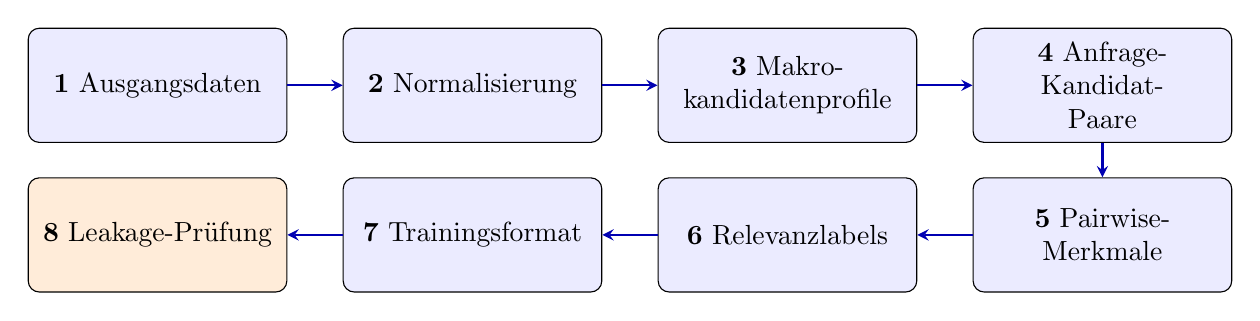
\begin{tikzpicture}[
        label distance=0.2cm,
        >=stealth,
        font=\normalsize,
        pipelinebox/.style={draw, rounded corners, fill=blue!8, text width=3.05cm, minimum height=1.45cm, inner ysep=0pt, align=center},
        check/.style={draw, rounded corners, fill=orange!15, text width=3.05cm, minimum height=1.45cm, inner ysep=0pt, align=center},
        flow/.style={->, thick, blue!70!black}
    ]
        \node[pipelinebox] (raw) at (0, 0) {\textbf{1} Ausgangsdaten};
        \node[pipelinebox] (norm) at (4.0, 0) {\textbf{2} Normalisierung};
        \node[pipelinebox] (profiles) at (8.0, 0) {\textbf{3} Makro-\\kandidatenprofile};
        \node[pipelinebox] (pairs) at (12.0, 0) {\textbf{4} Anfrage-Kandidat-\\Paare};

        \node[pipelinebox] (features) at (12.0, -1.9) {\textbf{5} Pairwise-\\Merkmale};
        \node[pipelinebox] (labels) at (8.0, -1.9) {\textbf{6} Relevanzlabels};
        \node[pipelinebox] (format) at (4.0, -1.9) {\textbf{7} Trainingsformat};
        \node[check] (leakage) at (0, -1.9) {\textbf{8} Leakage-Prüfung};

        \draw[flow] (raw) -- (norm);
        \draw[flow] (norm) -- (profiles);
        \draw[flow] (profiles) -- (pairs);
        \draw[flow] (pairs) -- (features);
        \draw[flow] (features) -- (labels);
        \draw[flow] (labels) -- (format);
        \draw[flow] (format) -- (leakage);
    \end{tikzpicture}
    \caption{Verarbeitungsschritte von den Ausgangsdaten bis zum Trainingsformat.}
    \label{fig:trainingsformat_pipeline}
\end{figure}

\chapter{Datensplit und Training} 
\label{chap:datensplit_und_training}

\section{Anforderungen an die Datenbasis}

Um eine konsistente, validierte und reproduzierbare Datenbasis zu haben, wurde ein idealer Datensatz erstellt.
Der ideale Datensatz setzt sich aus den bestgeeigneten Artikeln und Makrokandidaten nach der Datenbereinigung zusammen \parencite{srcIdealDataset,srcStep913}.
Dabei wurden die Anforderungen an den idealen Datensatz in Tabelle \ref{tab:anforderungen_datenbasis} zusammengefasst.

\begin{table}[tbp]
    \centering
    \setlength{\tabcolsep}{6pt}
    \renewcommand{\arraystretch}{1.08}
    \caption{Anforderungen an den idealen Datensatz \parencite{srcIdealDataset,srcStep913,srcStep921}}
    \label{tab:anforderungen_datenbasis}
    \begin{tabularx}{\textwidth}{>{\raggedright\arraybackslash}p{4.2cm} >{\raggedright\arraybackslash}X}
        \toprule
        \textbf{Anforderung} & \textbf{Beschreibung und Zielsetzung} \\
        \midrule
        Reale Datenbasis & Der Datensatz enthält ausschließlich tatsächlich vorhandene EPLAN-Artikel aus der gesamten Datenbasis. \\
        Eindeutiges Zielmakro & Jeder Artikel muss eindeutig einem Zielmakro (\texttt{target\_macro}) zugeordnet sein. \\
        Vorhandene Ground Truth & Für jedes Zielmakro muss eine passende reale \texttt{.ema}-Makrodatei existieren. \\
        Vollständige technische Merkmale & Die Feature-Vektoren müssen vorhanden und mit technischen Informationen gefüllt sein. \\
        Vollständige Grunddaten & Jeder Datensatz benötigt eine ID, ein Zielmakro, eine Makrofamilie und einen Fingerprint. \\
        Keine Duplikate & Artikel-IDs dürfen nicht mehrfach vorkommen, damit kein Artikel versehentlich doppelt trainiert wird. \\
        Keine widersprüchlichen Fingerprints & Ein Fingerprint darf nicht zu mehreren unterschiedlichen Zielmakros gehören. Andernfalls wäre die Zuordnung technisch nicht eindeutig. \\
        Ausgeglichener Target-Support & Jedes Zielmakro sollte ungefähr gleich häufig vertreten sein. Dadurch lernt das Modell nicht überwiegend die am häufigsten vorkommenden Makros. \\
        Vergleichbare Makrofamilien & Der Datensatz sollte mehrere Zielmakros derselben Familie enthalten. So kann geprüft werden, ob das Modell auch zwischen ähnlichen Makros unterscheiden kann. \\
        Leakage-freie und reproduzierbare Aufteilung & Die Daten werden mit einem festen Zufallswert (\texttt{RANDOM\_SEED} = 42) in 70\,\% Training, 10\,\% Validierung und 20\,\% Test aufgeteilt. Artikel mit zusammengehörigem Fingerprint bleiben dabei im selben Teil des Datensatzes \parencite{srcStep921}.\\
        \bottomrule
    \end{tabularx}
\end{table}

\section{Datensplit und Trainingsbasis}

Nach der Datenaufbereitung, der Qualitätsprüfung der Daten sowie der Erstellung des idealen Datensatzes erfolgt die Aufteilung in Trainings-, Validierungs- und Testdaten \parencite{srcStep911,srcStep913,srcIdealDataset,srcStep921}.
Ziel ist es eine klare Trennung zwischen Modelltraining, Hyperparameteroptimierung und Modellbewertung zu schaffen. 

\begin{align}
    \text{Train} = 70\,\%, \qquad \text{Validation} = 10\,\%, \qquad \text{Test} = 20\,\%
\end{align}

Um reproduzierbare Ergebnisse mit einem erstellten Datensplit zu gewährleisten, wird ein fester Zufallsseed verwendet, der sicherstellt, dass die Aufteilung in Trainings-, Validierungs- und Testdaten bei jeder Ausführung identisch bleibt \parencite{srcStep921}.

\begin{align}
    \text{RANDOM\_SEED} = 42
\end{align}

Dabei wird keine reine Zufallsaufteilung vorgenommen, sondern fachliche Zusammenhänge der Daten berücksichtigt, um eine konsistente Verteilung über die Anfragegruppen sicherzustellen. 
Dies verhindert, dass eng verwandte Beispiele in unterschiedlichen Datensplits landen und somit die Glaubwürdigkeit der Modellbewertung negativ beeinflussen. Durch die unterschiedlichen Seed-Werte lässt sich dann auch ein Mittelwert über mehrere Splits ableiten \parencite{srcStep921}. Abbildung \ref{fig:datensplit_schema} fasst diese Aufteilung schematisch zusammen.

\begin{figure}[tbp]
    \centering
    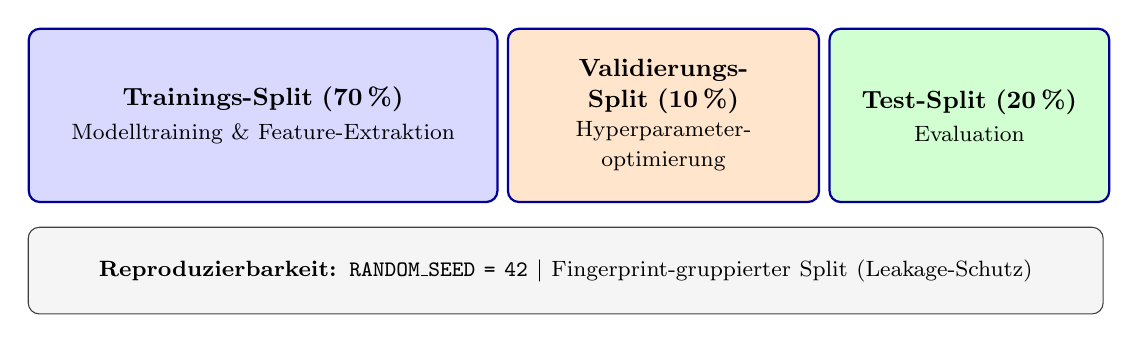
\begin{tikzpicture}[
        font=\small,
        bar/.style={draw=blue!60!black, thick, rounded corners=4pt, align=center, minimum height=2.2cm, inner sep=5pt},
        seed/.style={draw=gray!50!black, rounded corners=4pt, fill=gray!8, align=center, minimum height=1.1cm, inner sep=5pt}
    ]
        \node[bar, fill=blue!15, text width=5.6cm] (train) at (0,0) {\textbf{Trainings-Split (70\,\%)}\\[1pt]\footnotesize Modelltraining \& Feature-Extraktion};
        \node[bar, fill=orange!20, text width=3.6cm, right=3pt of train] (val) {\textbf{Validierungs-Split (10\,\%)}\\[1pt]\footnotesize Hyperparameter-\\optimierung};
        \node[bar, fill=green!18, text width=3.2cm, right=3pt of val] (test) {\textbf{Test-Split (20\,\%)}\\[1pt]\footnotesize Evaluation};

        \node[seed, below=0.3cm of train.south west, anchor=north west, text width=13.3cm] (seedbox) {\footnotesize \textbf{Reproduzierbarkeit:} \texttt{RANDOM\_SEED = 42} $\mid$ Fingerprint-gruppierter Split (Leakage-Schutz)};
    \end{tikzpicture}
    \caption{Schematische Aufteilung der Trainings-, Validierungs- und Testdatenbasis.}
    \label{fig:datensplit_schema}
\end{figure}

\section{Aufbau der Retrievalsignale}

Vor dem Modelltraining werden für jede Anfrage unterschiedliche Retrievalsignale berechnet (siehe Kapitel \ref{chap:analyse_der_datenstrukturen}) \parencite{srcStep640}.
Diese dienen als erste Ähnlichkeitsabschätzung zwischen Anfrage und Kandidat.

Die theoretischen Grundlagen der verwendeten Verfahren wurden bereits im Kapitel \ref{chap:stand_der_technik} beschrieben.
Die Retrievalsignale dienen innerhalb der in Abbildung \ref{fig:architektur} dargestellten Pipeline-Architektur nicht als eigenständige Rankingstufen, sondern als zusätzliche Merkmale für das Learning-to-Rank-Modell \parencite{srcStep640,srcStep931}.

Die folgende Tabelle \ref{tab:retrieval_signale} zeigt die verwendeten Retrievalsignale sowie deren Funktion.

\begin{table}[tbp]
    \centering
    \setlength{\tabcolsep}{6pt}
    \renewcommand{\arraystretch}{1.1}
    \caption{Verwendete Retrievalsignale} 
    \label{tab:retrieval_signale} 
    \begin{tabularx}{\textwidth}{>{\raggedright\arraybackslash}p{3.5cm} >{\raggedright\arraybackslash}X}
        \toprule
        \textbf{Signal} & \textbf{Funktion} \\
        \midrule
        BM25 & Lexikalische Ähnlichkeit zwischen Anfrage und Makrokandidatenprofil \\
        Exact Match & Exakte technische Übereinstimmungen strukturierter Merkmale \\
        RRF & Fusion der Retrievalrankings zu einem kombinierten Retrievalsignal \\
        \bottomrule 
    \end{tabularx}
\end{table}


Die verwendeten Parameter der Retrievalkomponenten wurden wie folgt festgelegt \parencite{srcStep640}:

\begin{align}
    \text{BM25}_{k1} &= 1.2 \\
    \text{BM25}_{b}  &= 0.50 \\
    \text{RRF}_{k}   &= 30
\end{align}

Dabei steuert $k_1$ wie stark wiederholte Treffer eines Begriffes berücksichtigt werden. Hier wurden 1,2 gewählt, da sich wiederholende lexikalische Begriffe zwar relevant sein können,
aber nicht automatisch bedeuten, das ein EPLAN-Artikel \parencite{EPLANArtikelverwaltung} für ein EPLAN-Fenstermakro \parencite{EPLAN-Makros} relevanter ist.

Der Parameter $b$ steuert die Normalisierung der Dokumentenlänge. Dieser liegt zwischen 0 und 1 und wurde hier auf 0,50 gesetzt. Dadurch wird berücksichtigt, dass längere Kandidatenprofile mehr Treffer enthalten können,
diese aber nicht aufgrund der Länge einen übermäßigen Vorteil erhalten \parencite{srcStep640}.

$\text{RRF}_k$ steuert den Einfluss der Spitzenpositionen. Bei kleinem $k$ dominiert Rang 1 stark, während bei größerem $k$ auch niedrigere Ränge stärker berücksichtigt werden.
60 ist die übliche Wahl. Hier wurde 30 verwendet, um die Spitzenpositionen nicht zu stark zu reduzieren und damit dem Ranking auf Top 1 mehr Abstand zu verleihen \parencite{srcStep640}.

Die Fusion der Retrievalsignale erfolgt über die Gewichtung der Reciprocal Rank Fusion (RRF) \parencite{srcStep640}:

\begin{align}
    w_{\text{BM25}} = 0.30 \qquad \text{und} \qquad w_{\text{Exact}} = 0.70
\end{align}

Die höhere Gewichtung von Exact Match gegenüber BM25 spiegelt die Priorität technischer Merkmale innerhalb der Maschinen- und Anlagenbau-Domäne wider. 


\section{Training des Learning-to-Rank-Modells}

Das zentrale Element der Architektur ist das Learning-to-Rank-Modell. Hierfür wird der \texttt{LGBMRanker} der LightGBM-Bibliothek verwendet \parencite{srcStep931}.
Dieser basiert auf dem in Kapitel \ref{chap:stand_der_technik} beschriebenen LambdaRank-/LambdaMART-Prinzip.

Das Modell wird mit den Parametern 

\begin{align} 
    \text{objective} = \text{lambdarank} \qquad \text{und} \qquad \text{metric} = \text{ndcg}
\end{align} 

trainiert \parencite{srcStep931}.


Wie in Kapitel \ref{chap:analyse_der_datenstrukturen} beschrieben, werden Kandidaten einer Anfrage als gemeinsame Rankinggruppe betrachtet.
Wiederholend entsteht für jede Anfrage eine Gruppe:

\begin{align} 
    G_q = \{(q,c_1),(q,c_2),\dots,(q,c_n)\} 
\end{align} 

mit der Anfrage $q$ und den zugehörigen Makrokandidaten $c_i$.

Dadurch erlernt das Modell nicht die allgemeine Zugehörigkeit eines einzelnen Kandidaten zu einer Klasse. Stattdessen wird die optimale Kandidatenreihenfolge innerhalb derselben Anfrage gelernt.
Ziel dabei ist es, dass der relevanteste Kandidat möglichst weit oben in der Rangliste erscheint.

Die Eingaben für das Modell sind die im Kapitel \ref{chap:analyse_der_datenstrukturen} beschriebenen Pairwise-Merkmale.
Das Training erfolgt dabei ausschließlich auf den Trainingsdaten, während die Optimierung der Hyperparameter über die Validierungsdaten erfolgt \parencite{srcStep931}.

\section{Hyperparameteroptimierung}

Die Leistungsfähigkeit eines Learning-to-Rank-Modells hängt von der Wahl der Hyperparameter ab. Deswegen erfolgt die Modellkonfiguration nicht manuell, sondern durch eine systematische Hyperparameteroptimierung.
Dafür wird hier eine Grid-Search-basierte Strategie verwendet. Bei dieser werden verschiedene Kombinationen von Hyperparametern getestet und anhand der Ergebnisse der Validierung verglichen \parencite{srcStep931}.

Die folgende Tabelle \ref{tab:hyperparameter} zeigt die untersuchten Hyperparameterkombinationen:

\begin{table}[tbp] 
    \centering 
    \setlength{\tabcolsep}{8pt}
    \renewcommand{\arraystretch}{1.1}
    \caption{Verwendete Hyperparameterkombinationen \parencite{srcStep931}}
    \label{tab:hyperparameter} 
    \begin{tabularx}{0.85\textwidth}{>{\raggedright\arraybackslash}p{5.5cm} >{\raggedright\arraybackslash}X} 
        \toprule 
        \textbf{Parameter} & \textbf{Wertebereich} \\ 
        \midrule 
        \texttt{n\_estimators} & 300, 500, 700 \\ 
        \texttt{learning\_rate} & 0.05, 0.04, 0.035 \\ 
        \texttt{num\_leaves} & 31, 63 \\ 
        \texttt{min\_child\_samples} & 10, 20, 50 \\ 
        \texttt{lambdarank\_\allowbreak truncation\_level} & 10, 20 \\ 
        \bottomrule 
    \end{tabularx} 
\end{table}

Dabei sind die Hyperparameter wie folgt zu verstehen:

\begin{itemize}
    \item \textbf{\texttt{n\_estimators}:} Anzahl der aufgebauten Entscheidungsbäume im Modell. Mehr Bäume = komplexere Zusammenhänge, aber mehr Rechenaufwand.
    \item \textbf{\texttt{learning\_rate}:} Lernrate pro Trainingsschritt. Kleinere Werte führen zu vorsichtigerem, aber stabileren Lernen.
    \item \textbf{\texttt{num\_leaves}:} Maximale Anzahl der Blätter pro Baum. Mehr Blätter = komplexere Bäume, aber höheres Risiko für Overfitting.
    \item \textbf{\texttt{min\_child\_samples}:} Minimale Anzahl an Trainingsbeispielen in einem Blatt. Kleinere Werte = mehr Detailtreue pro Blatt, größere Werte = bessere Regularisierung (verhindert Overfitting).
    \item \textbf{\texttt{lambdarank\_\allowbreak truncation\_level}:} Begrenzung des Ranglistenbereichs, der durch LambdaRank optimiert werden soll (Top 10, Top 20).
\end{itemize}

Für jede Parameterkombination wird ein vollständiger Trainingsdurchlauf durchgeführt. Die Bewertung erfolgt anschließend auf dem Validierungsdatensatz.
Das finale Modell wird auf Basis der Rankingqualität anhand der Validierungsdaten bestimmt \parencite{srcStep931}.

Die verwendeten Bewertungsmetriken werden später in Kapitel \ref{chap:evaluierungskonzept_und_ergebnisse} ausführlich beschrieben.

\section{Modellartefakte und Reproduzierbarkeit}

Ein wichtiges Ziel dieser Trainingspipeline besteht darin, die Trainingsabläufe reproduzierbar zu gestalten. Deswegen werden nach jedem Trainingslauf alle relevanten Artefakte gespeichert und dokumentiert \parencite{srcStep931}. Abbildung \ref{fig:artefakte_struktur} zeigt die zugehörige Ablagestruktur.

\begin{figure}[tbp]
    \centering
    \begin{tikzpicture}[
        font=\small,
        dirbox/.style={draw=blue!60!black, thick, rounded corners, fill=blue!5, text width=4.8cm, align=left, inner sep=6pt},
        artbox/.style={draw=teal!60!black, thick, rounded corners, fill=teal!5, text width=7.0cm, align=left, inner sep=6pt}
    ]
        \node[dirbox] (dir) {
            \textbf{Ablagestruktur im Laufverzeichnis:}\\[4pt]
            \ttfamily\small
            run\_directory/\\
            $\text{\textbar}$-- model/\\
            $\text{\textbar}$-- training/\\
            $\text{\textbar}$-- evaluation/\\
            $\text{\textbar}$-- summary/\\
            $\text{\textbackslash}$-- error\_analysis/
        };
        \node[artbox, right=0.5cm of dir] (art) {
            \textbf{Gespeicherte Modellartefakte:}\\[4pt]
            \small
            \begin{itemize}[leftmargin=12pt, itemsep=2pt, topsep=0pt]
                \item das trainierte LightGBM-Modell,
                \item die verwendeten Hyperparameter,
                \item die erzielten Validierungsmetriken,
                \item die verwendeten Featuredefinitionen,
                \item die Makrokandidatenprofile,
                \item Konfigurations- und Laufmetadaten.
            \end{itemize}
        };
    \end{tikzpicture}
    \caption{Strukturierte Ablage der Modellartefakte im Laufverzeichnis.}
    \label{fig:artefakte_struktur}
\end{figure}

Dadurch lässt sich sicherstellen, dass jeder Trainingsablauf zu einem späteren Zeitpunkt vollständig nachvollzogen und reproduziert werden kann \parencite{srcStep931}.


\section{Pipeline-Orchestrierung}

Die Ausführung der gesamten Pipeline erfolgt über eine zentrale Komponente, die die Orchestrierung übernimmt. 
Dadurch wird sichergestellt, dass alle Verarbeitungsschritte in der richtigen Reihenfolge ausgeführt werden \parencite{srcStep936}.

Die folgende Reihenfolge der Schritte stellt den Ablauf der Pipeline dar. Diese können auch aus dem Architekturdiagramm in Abbildung \ref{fig:architektur} entnommen werden:

\begin{enumerate} 
    \item Datenaufbereitung 
    \item Qualitätsprüfung und Datenvalidierung 
    \item Datensplit   
    \item Berechnung der Retrievalsignale 
    \item Erstellung der Pairwise-Features 
    \item Training des Rankingmodells 
    \item Speicherung der Modellartefakte 
    \item Evaluation des trainierten Modells 
\end{enumerate}

Jeder Verarbeitungsschritt verwendet dabei die Artefakte des vorherigen Schrittes als Eingabe und erzeugt selbst Artefakte für den nächsten Schritt als Ausgabe. 
Dadurch wird ein konsistenter Datenfluss von den Roh-Daten bis zum trainierten Modell sichergestellt \parencite{srcStep936,srcPipeline}.
\chapter{Evaluierungskonzept}
\label{chap:evaluierungskonzept}

\section{Evaluationsdatensätze}

Die Bewertung der Modelleistung erfolgt getrennt auf Trainings-, Validierungs- und Testdatensätzen.
Diese Aufteilung wird im Rahmen des zuvor beschriebenen Kapitels \ref{chap:datensplit_und_training} vorgenommen.

Der Testdatensatz wird erst nach der finalen Modellauswahl für die abschließenden Evaluierungen verwendet.
Dadurch wird verhindert, dass Informationen aus dem Testdatensatz in die Optimierung des Modells einfließen und die Bewertung verfälschen.

Ein wichtiger Aspekt dabei ist die Behandlung von fachlich Zusammenhängenden Daten. Artikel die denselben Fingerprint besitzen, dürfen nur gemeinsam in einem Teil des Splits vorkommen.
Ein Fingerprint repräsentiert die Struktur und die wesentlichen Merkmale eines Artikels, sodass Artikel mit demselben Fingerprint als fachlich zusammenhängend betrachtet werden.

Dadurch wird verhindert, dass nahezu ähnliche Beispiele gleichzeitig im Trainings- und Testdatensatz vorkommen.

\section{Aufbau der Evaluations-Suite} 

Die Evaluation des Learning-to-Rank-Modells erfolgt automatisiert mithilfe einer Evaluations-Suite \parencite{srcEvalSuite}, welche in dem Modul \texttt{step\_944\_analyze\_ltr\_run.py} verankert ist.
Damit wertet das Modul die Vorhersagen des trainierten Modells auf dem Validierungs- und Testdatensatz aus und berechnet die definierten Rankingmetriken sowie zusätzliche Fehleranalysen.

\begin{table}[tbp] 
  \centering 
  \caption{Aktuelle Evaluations-Suite} 
  \label{tab:evaluations_suite} \begin{tabularx}{\textwidth}{p{1cm}p{5cm}X} 
    \toprule 
    \textbf{Nr.} & \textbf{Skript} & \textbf{Zielsetzung} \\ 
    \midrule 1 & \texttt{step\_944\_analyze\_ltr\_run.py} & Berechnung der Rankingmetriken, Fehleranalyse und Evaluationsstatistiken \\ 
    \bottomrule 
  \end{tabularx} 
\end{table}

Die Ergebnisse dieser Pipeline werden strukturiert in den folgenden Verzeichnissen abgelegt:

\begin{itemize}
  \item \texttt{evaluation/step\_941\_leakage\_safety} für die Prüfung auf Zielinformations-Leakage
  \item \texttt{evaluation/step\_942\_retrieval\_validation} für die Bewertung des Retrieval-Index
  \item \texttt{evaluation/step\_943\_candidate\_coverage} für die Analyse der Kandidatenabdeckung
  \item \texttt{evaluation/step\_944\_ltr\_run\_analysis} für die Analyse des Learning-to-Rank-Modells
\end{itemize}

\section{Verwendete Rankingmetriken} 

Die theoretischen Grundlagen der verwendeten Rankingmetriken wurden bereits in Kapitel \ref{chap:stand_der_technik} behandelt. 
Für die Bewertung des Systems aus dieser Arbeit werden die folgenden Kennzahlen verwendet: 

\begin{itemize} 
  \item Target Recall@1, @3, @5 und @10 
  \item Family Recall@1, @3, @5 und @10 
  \item Mean Reciprocal Rank (MRR) 
  \item Hierarchical nDCG@1, @3, @5 und @10 
  \item Rangstatistiken der Ziel-Makros \parencite{EPLAN-Makros} 
\end{itemize} 

Durch diese Metriken können die Zielmakroerkennung, der Familienerkennung sowie die allgemeinen Rankingqualität bewertet werden.

\subsection{Bedeutung der Metriken innerhalb der Evaluation} 

Die Bewertungsmetriken bilden gemeinsam verschiedene Aspekte der Rankingqualität ab, wie in Tabelle \ref{tab:rankingmetriken_bedeutung} zusammengefasst.

\begin{table}[tbp]
  \centering
  \setlength{\tabcolsep}{6pt}
  \renewcommand{\arraystretch}{1.1}
  \caption{Bedeutung der verwendeten Rankingmetriken}
  \label{tab:rankingmetriken_bedeutung}
  \begin{tabularx}{\textwidth}{>{\raggedright\arraybackslash}p{4cm} >{\raggedright\arraybackslash}X}
    \toprule
    \textbf{Metrik} & \textbf{Bewerteter Qualitätsaspekt} \\
    \midrule
    Target Recall@k & Position des exakten Ziel-Makros \parencite{EPLAN-Makros} \\
    Family Recall@k & Erkennung der korrekten Makrofamilie \\
    MRR & Durchschnittlicher Zielrang \\
    Hierarchical nDCG & Qualität der gesamten Rangfolge \\
    \bottomrule
  \end{tabularx}
\end{table}


\section{Leakage-Sicherheitsprüfung}

Ein zentraler Bestandteil in der Evaluation ist eine Leakage-Sicherheitsprüfung auf Zielinformationen. 
Unter Leakage wird die unbeabsichtigte Nutzung von Informationen verstanden, die zum Zeitpunkt einer realen Vorhersage nicht verfügbar sein dürften und dadurch zu unrealistisch guten Modellergebnissen führen würden \parencite{kaufman2012leakage}.
Da dieses System auf Artikel \parencite{EPLANArtikelverwaltung} - Makro \parencite{EPLAN-Makros} -Zuordnungen trainiert wird, besteht das Risiko, 
das Informationen über das tatsächliche Ziel-Makro \parencite{EPLAN-Makros} in die Trainings- und Evaluierungsdaten gelangen können und somit die Aussagekraft der verwendeten Evaluationsmetriken verfälscht wird.

Um dies zu vermeiden, enthält die Pipeline eine Leakage-Prüfung, die vor der eigentlichen Modellbewertung ausgeführt wird.
Die Implementierung erfolgt in \texttt{step\_941\_\allowbreak validate\_leakage\_\allowbreak safety.py} \parencite{srcStep941}.

\subsection{Ziele der Leakage-Prüfung}

Die Ziele der Leakage-Prüfung sind:

\begin{itemize} 
\item Identifikation verbotener Zielinformationen innerhalb der Query-Daten 
\item Erkennung direkter Ziel-Makro \parencite{EPLAN-Makros} -Referenzen 
\item Prüfung auf Familien- und Zielinformationen innerhalb von Eingangsmerkmalen 
\item Kontrolle der Kandidatenprofile 
\item Überprüfung der Datensplits auf Überschneidungen 
\item Sicherstellung der Trennung von Training, Validierung und Test 
\end{itemize}

Somit wird sichergestellt, dass das Modelltraining nur mit den Informationen erfolgt, die später auch im Produktivbetrieb verfügbar sind.

\subsection{Prüfung der Query-Daten}

Die verwendete Query-Darstellung repräsentiert einen eingehenden Artikel \parencite{EPLANArtikelverwaltung} beziehungsweise die Informationen aus einem Datenblatt, die für eine Suchanfrage an das trainierte Modell wichtig sind.

Wichtig hierbei ist es, dass keine direkten Hinweise auf das Ziel-Makro \parencite{EPLAN-Makros} in den Query-Daten enthalten sind, welche unmittelbar auf dieses verweisen können.

Deswegen untersucht die Leakage-Prüfung folgenden Punkte:

\begin{itemize} 
  \item Ziel-Makro \parencite{EPLAN-Makros} -Kennungen 
  \item Zielfamilieninformationen 
  \item direkten Ziel-Makro \parencite{EPLAN-Makros} -Tokens 
  \item verbotenen Metadatenfeldern 
  \item impliziten Zielhinweisen in den Featurevektoren 
\end{itemize}

Sobald solche Informationen gefunden werden, wird der Lauf als Ungültig markiert.

\subsection{Prüfung der Datensplits}

Neben der Query-Prüfung erfolgt auch eine Prüfung des erzeugten Datensplits. Dabei wird überprüft, ob unerlaubte Überschneidungen zwischen Training, Validierung und Test vorhanden sind.

Dabei werden folgende Aspekte überprüft:

\begin{itemize} 
  \item Fingerprint-Gruppen 
  \item Fenstermakrozuordnungen \parencite{EPLAN-Makros} 
  \item Kandidatenprofile 
  \item technische Zusammenhangskomponenten 
  \item gruppierte Artikelstrukturen 
\end{itemize}

Das Ziel dieser Prüfung ist es, sicherzustellen, dass keine fachlich identischen Beispiele gleichzeitig in mehreren Datensplits vorhanden sind. Dadurch wird ein künstliche Modell-Verbesserung verhindert,
die die Generalisierungsfähigkeit des Modells beeinträchtigen würde.

\subsection{Prüfung der Kandidatenprofile}

Ein weiterer Bereich der Prüfung betrifft die Makro-Kandidatenprofile \parencite{EPLAN-Makros}.
Da diese Profile aus den Trainingsdaten entstehen, muss sichergestellt werden, dass keine Informationen aus den Validierungs- oder Testdaten in die Kandidatenprofile einfließen.

Deswegen werden sämtliche Profilinformationen auf ihre Herkunft geprüft, um sicherzustellen, dass ausschließlich Daten des Trainingssplits zur Erstellung der Kandidatenprofile verwendet werden \parencite{srcLeakageGuard}.

\subsection{Evaluierungsergebnis}

Nach der Leakage-Prüfung wird ein struktruierter Sicherheitsbericht erstellt. Der Evaluationslauf gilt nur dann als bestanden, wenn keine Verstöße gegen die definierten Leakage-Regeln festgestellt wurden.
Diese Basis bildet die Voraussetzung für die Interpretierbarkeit der nachfolgenden Rankingmetriken.

Für den verwendeten Datensatz wurden keine Fingerprint-Konflikte noch Fingerprint-Leaks festgestellt. 
Es sind auch keine Ziel-Makros \parencite{EPLAN-Makros} oder Makrofamilien in Validierungs- beziehungsweise Testdaten vorhanden, ohne zuvor im Trainingssplit vertreten zu sein. 


\chapter{Ergebnisse und Diskussion}
\label{chap:ergebnisse_und_diskussion}

\section{Ergebnisse des Validierungssplits}

Die Ergebnisse des Validierungssplits werden im späteren Verlauf für die Auswahl der besten Modellkonfiguration verwendet.

Tabelle \ref{tab:validation_ergebnisse} fasst die wichtigsten Rankingmetriken des Referenzlaufs A08 auf dem Validierungssplit zusammen. 

\begin{table}[tbp] 
  \centering 
  \caption{Ergebnisse des Referenzlaufs A08 auf dem Validierungssplit} 
  \label{tab:validation_ergebnisse} 
  \begin{tabular}{lr} \toprule \textbf{Metrik} & \textbf{Wert} \\ 
    \midrule 
    Target Recall@1 & 0,3137 \\
    Target Recall@3 & 0,4472 \\
    Target Recall@5 & 0,5031 \\
    Target Recall@10 & 0,6211 \\
    Family Recall@1 & 0,8199 \\
    Family Recall@10 & 0,8913 \\
    MRR & 0,4121 \\
    Hierarchical nDCG@10 & 0,6766 \\
    \bottomrule 
  \end{tabular} 
\end{table}

Die Ergebnisse zeigen, dass das Modell bereits nach dem Test durch den Validierungssplit die korrekte Makrofamilie besser identifiziert als die exakte Ziel-Makro \parencite{EPLAN-Makros}.
Während das korrekte Ziel-Makro \parencite{EPLAN-Makros} in 31,37\,\% der Anfragen auf Platz 1 steht, wird die korrekte Makrofamilie in 81,99\,\% der Anfragen auf die erste Position gesetzt.

Durch den Target Recall@10 lässt sich erkennen, dass das Modell in 62,11\,\% der Anfragen das korrekte Ziel-Makro \parencite{EPLAN-Makros} innerhalb der Top-10-Vorschläge platziert.
Interessant ist der Abstand zwischen Family Recall@10 (89,13\,\%) und Target Recall@10 (62,11\,\%). Dies deutet darauf hin, dass viele Fehlkategorisierungen innerhalb derselben Makrofamilie stattfinden.

Die erzielten Ergebnisse bei MRR von 0,4121\,\% sowie ein hierarchisches nDCG@10 von 0,6766\,\%  zeigen zusätzlich, dass beim Validierungssplit das Modell in der Lage ist eine sinnvolle Reihenfolge zu erzeugen, 
es jedoch weiterhin Schwierigkeiten bei der korrekten Auflösung technischer Varianten besitzt.\parencite{LTR_Configuration_Test_Series}

\section{Ergebnisse des Testsplits}

Nach dem die Modellauswahl abgeschlossen wurde, erfolgt die finale Evaluation des ausgewählten Modells auf dem unberührten Testsplit.

Tabelle \ref{tab:test_ergebnisse} zeigt die erzielten Ergebnisse des Referenzlaufs A08 des Testsplits. 

\begin{table}[tbp] 
  \centering 
  \caption{Ergebnisse des Referenzlaufs A08 auf dem Testsplit} 
  \label{tab:test_ergebnisse} 
  \begin{tabular}{lr} \toprule \textbf{Metrik} & \textbf{Wert} \\ \midrule 
    Target Recall@1 & 0,3478 \\
    Target Recall@3 & 0,4783 \\
    Target Recall@5 & 0,5494 \\
    Target Recall@10 & 0,6798 \\
    Family Recall@1 & 0,8735 \\
    Family Recall@10 & 0,9368 \\
    MRR & 0,4534 \\
    Hierarchical nDCG@10 & 0,7449 \\
    \bottomrule 
  \end{tabular} 
\end{table}

Beim Testsplit zeigt sich ein ähnliches Bild wie beim Validierungssplit. Das Modell sagt bei 34,78\,\% der Anfragen das korrekte Ziel-Makro \parencite{EPLAN-Makros} auf Platz 1 voraus, während die korrekte Makrofamilie in 87,35\,\% der Anfragen auf die erste Position gesetzt wird.

Wie beim Validierungsplit ist auch hier der deutliche Abstand zwischen Family Recall@10 (93,68\,\%) und Target Recall@10 (67,98\,\%) zu erkennen. 

Der erreichte MRR- Wert von 45,34\,\% sowie die hierarchische nDCG@10 von 74,49\,\% bestätigen zusätzlich die Erkenntnisse aus dem Validierungssplit.\parencite{LTR_Configuration_Test_Series}

\section{Fehleranalyse}

Um die Modellleistung detailliert erfassen zu können, werden die Top-1-Ergebnisse des Testsplits analysiert. Dabei werden die fachlichen Beziehungen zum tatsächlichen Zielmakro untersucht.

Tabelle \ref{tab:fehleranalyse_top1} zeigt die Verteilung der einzelnen Fehlerkategorien. 

\begin{table}[tbp] 
  \centering 
  \caption{Top-1-Analyse der Vorhersagen auf dem Testdatensatz} 
  \label{tab:fehleranalyse_top1} 
  \begin{tabular}{lrr} 
    \toprule 
    \textbf{Kategorie} & \textbf{Anzahl} & \textbf{Anteil} \\ 
    \midrule 
    Exaktes Ziel-Makro \parencite{EPLAN-Makros} & 88 & 34,78\,\% \\
    Gleiche Familie, falsches Target & 133 & 52,57\,\% \\
    Gleicher Familienpräfix & 12 & 4,74\,\% \\
    Andere Familie & 20 & 7,91\,\% \\
    \bottomrule 
  \end{tabular} 
\end{table}

Die Fehleranalyse bestätigt die Beobachtungen aus den Metriken. Von insgesamt 253 Testanfragen werden 133 Fälle einer gleichen Familie, aber einer falschen Variante zugeordnet, was 52,57\,\% entspricht.
In 7,91\,\% der Fälle wird eine andere Familie vorhergesagt. Das zeigt, dass das Modell die grundlegenden technischen Zusammenhänge zwischen Artikeln und Makrofamilien zuverlässig erlernt hat.
Die Analyse zeigt, dass die zentrale Herausforderung die Identifikation des korrekten Ziel-Makros \parencite{EPLAN-Makros} innerhalb der richtigen Makrofamilie ist. Dafür muss die Variantenauflösung innerhalb der Makrofamilie weiter verbessert werden.
Die große Differenz zwischen dem Target Recall@1 und dem Family Recall@1 unterstreicht diese Herausforderung zusätzlich.
Dies wird im Kapitel \ref{chap:grenzen_und_ausblick} genauer analysiert.\parencite{LTR_Configuration_Test_Series}


\section{Rangstatistische Analyse}

Eine weitere wichtige Analyse ist die statistische Auswertung der erzeugten Ranglisten.


Die wichtigsten Rangstatistiken des Testdatensatzes werden in Tabelle \ref{tab:rangstatistik} dargestellt.

\begin{table}[tbp] 
  \centering 
  \caption{Rangstatistische Kennzahlen des Testsplits} 
  \label{tab:rangstatistik} 
  \begin{tabular}{lr} 
    \toprule 
    \textbf{Kennzahl} & \textbf{Wert} \\ 
    \midrule 
    Erwarteter Zielrang (Mean Rank) & 23,96 \\
    Median Rank & 4 \\
    90\,\%-Perzentil Rank & 61,6 \\
    Maximaler Rang & 360 \\
    \bottomrule 
  \end{tabular} 
\end{table}

Der Median Rank von 4 zeigt, dass das korrekte Makro \parencite{EPLAN-Makros} in der Hälfte der Testanfragen unter den ersten vier Positionen der Rangliste erscheint.
Der mittlere Rang (Mean Rank) von 23,96 zeigt gleichzeitig, dass es einzelne schwierige Anfrage gibt, die deutliche schlechter eingeordnet werden.
Diese Annahme wird durch das 90\,\%-Perzentil von 61,6 bestätigt. Dabei sitzt das Makro \parencite{EPLAN-Makros} in 90\,\% der Testanfragen unter den ersten 61,6 Positionen der Rangliste.

Auch die Rangstatistiken zeigen, dass das Modell in der Lage ist, die korrekte Makro-Familie in den meisten Fällen weit oben in der Rangliste zu platzieren.\parencite{LTR_Configuration_Test_Series}

\section{Analyse der Generalisierungsfähigkeit}

Zur Beurteilung der Generalisierungsfähigkeit des Modells wurde eine zusätzliche Leave-One-Out Kontrollanalyse durchgeführt. 
Um eine Verfälschung der Ergebnisse der Trainingsanalyse zu verhindern, werden bei einer Anfrage genau dieser Artikel aus der Anfragemenge ausgeschlossen.


Tabelle \ref{tab:loo_vergleich} stellt die Ergebnisse der Leave-One-Out-Analyse (LOO) sowie der Validierungs- und Testergebnisse gegenüber.

\begin{table}[tbp] 
  \centering 
  \caption{Vergleich von regulärer Trainingsbewertung, Leave-One-Out-Analyse, Validation und Test} 
  \label{tab:loo_vergleich} 
  \begin{tabular}{lrrrr} 
    \toprule 
    \textbf{Metrik} & \textbf{Train (LOO)} & \textbf{Validation} & \textbf{Test} \\ 
    \midrule 
    Recall@1 & 0,1870 & 0,3137 & 0,3478 \\
    Recall@3 & 0,3028 & 0,4472 & 0,4783 \\
    Recall@10 & 0,4695 & 0,6211 & 0,6798 \\
    MRR & 0,2864 & 0,4121 & 0,4534 \\
    Family Recall@1 & 0,7246 & 0,8199 & 0,8735 \\
    Hierarchical nDCG@10 & 0,5945 & 0,6766 & 0,7449 \\
    Mean Rank & 25,93 & 23,96 & 23,96 \\
    Median Rank & 13,0 & 4,0 & 4,0 \\
    90\,\%-Perzentil & 62,0 & 61,6 & 61,6 \\
        \bottomrule 
    \end{tabular} 
    \end{table}

Es zeigt sich, dass die Leave-One-Out-Bewertung eine strengere Evaluationsmethode als die Bewertung durch den Validierungs- und Testdatensatz darstellt.
Die Ursache dafür liegt im Support der Kandidatenprofile. Von den vorhanden 375 Kandidatenprofilen basieren insgesamt 302 Profile ausschließlich auf einem Trainingsartikel.
Wenn dieser Artikel aus der Anfragemenge ausgeschlossen wird, enthält das entsprechende Kandidatenprofil keine unterstützenden Trainingsdaten mehr und kann dadurch keinen Beitrag zur korrekten Vorhersage leisten.

Bei den Validierungs- und Testdaten tritt dieser Effekt nicht auf, da durch die im Datensplit erzwungene Trainingsabdeckung jedes Ziel-Makro \parencite{EPLAN-Makros} mindestens einen Artikel in jedem Split enthält, welcher nicht identisch zu den andern beiden ist.


\section{Vergleich der Konfigurationsvarianten}

Um verschiedene Modellkonfigurationen zu vergleichen, wurde die aktuell Versuchsserie A01 bis A09 durchgeführt. 
Dabei wurden unterschiedliche Strategien, Profilbreiten und Regularisierungsparameter getestet. Ziel davon ist es, die Einflüsse einzelner Parameter auf die Modellleistung zu analysieren.\parencite{LTR_Configuration_Test_Series}

\subsection{Untersuchte Konfigurationsparameter}

Die verschiedenen Varianten der Konfiguration haben unterschiedliche Auswirkungen auf die Trainingslabels, die Kandidatenprofile sowie der Modellregularisierung. 
Die untersuchten Konfigurationsparameter werden in folgender Tabelle \ref{tab:konfigurationsparameter} erläutert.

\begin{table}[tbp] 
    \centering 
    \caption{Untersuchte Konfigurationsparameter} 
    \label{tab:konfigurationsparameter} 
    \begin{tabularx}{\textwidth}{p{4cm}X} 
        \toprule \textbf{Parameter} & \textbf{Bedeutung} \\ 
        Same-Family-Gewicht &  Negative Kandidaten aus derselben Makrofamilie werden innerhalb der Verlustfunktion unterschiedlich gewichtet. Dadurch kann die Variantenauflösung stärker betont werden. \\ 
        Profilbreite & Begrenzt die Anzahl der gespeicherten Profilwerte innerhalb eines Kandidatenprofils. Kleinere Profilbreiten erzeugen eine kompaktere Kandidatenrepräsentation. \\ 
        L1-Regularisierung ($\alpha$) & Bestraft große Modellgewichte und reduziert die Modellkomplexität. Dadurch werden irrelevante Merkmale stärker unterdrückt. \\ 
        L2-Regularisierung ($\lambda$) & Stabilisiert die Gewichtung der einzelnen Merkmale und reduziert die Gefahr einer Überanpassung an einzelne Trainingsbeispiele. \\ 
        Min. Split Gain & Definiert den minimal notwendigen Informationsgewinn um eine Baumaufteilung im LightGBM-Modell zu ermöglichen. Höhere Werte führen dadurch zu konservativeren Entscheidungsbäumen. \\ 
        \bottomrule 
    \end{tabularx} 
\end{table} 

A02 bis A07 wurden so gewählt, dass immer nur ein Parameter gezielt verändert wurde. Dadurch lassen sich die Auswirkungen der einzelnen Konfigurationsparameter isoliert untersuche.
Bei A08 und A09 werden mehrere Parameter (L1 und L2) gleichzeitig verändert, da diese bei LightGBM konzeptionell derselbe Hebel sind (Bestrafung der Blattgewichte). 
Um eine sinnvolle "stärkere Regularisierung" zu erzielen, ist es in der Praxis sinnvoll, beide gemeinsam hochzudrehen, nicht nur einen isoliert.
Bei A09 kommt zusätzlich ein positiver Wert für \texttt{min\_split\_gain} zum Einsatz um dadurch einen noch größeren Einfluss auf eine "stärkere Regularisierung" zu erzielen.\parencite{LTR_Configuration_Test_Series}


\subsection{Referenzkonfiguration A01}

A01 dient als Referenzkonfiguration und bildet die Basis für die Vergleichsexperimente. Sie enthält die Standardwerte für alle untersuchten Konfigurationsparameter.
Alle weiteren Konfigurationen A02 bis A09 werden gegenüber dieser bewertet.

Die Referenzparameter lauten: 

\begin{table}[tbp] 
    \centering 
    \caption{Referenzkonfiguration A01} 
    \label{tab:a01_referenz} 
    \begin{tabular}{ll} 
        \toprule 
        \textbf{Parameter} & \textbf{Wert} \\ 
        \midrule 
        Exaktes Targettraining & Ja \\ 
        Same-Family-Gewicht & 5,0 \\ 
        Profilbreite & 16 \\ 
        L1-Regularisierung ($\alpha$) & 0,05 \\ 
        L2-Regularisierung ($\lambda$) & 0,2 \\ 
        Min. Split Gain & 0,0 \\ 
        \bottomrule 
    \end{tabular} 
\end{table}

Ausgehen von dieser Basis werden die folgenden Varianten der Konfigurationen A02 bis A09 verändert.

Tabelle \ref{tab:konfigurationsabweichungen} zeigt die gegenüber A01 vorgenommenen Veränderungen. 
\begin{table}[tbp] 
    \centering 
    \caption{Abweichungen der Konfigurationen gegenüber der Referenz A01} 
    \label{tab:konfigurationsabweichungen} 
    \begin{tabular}{lp{8cm}} 
        \toprule 
        \textbf{Konfiguration} & \textbf{Änderung gegenüber A01} \\ 
        \midrule 
        A02 & Same-Family-Gewicht von 5,0 auf 2,0 reduziert \\ 
        A03 & Same-Family-Gewicht von 5,0 auf 8,0 erhöht \\ 
        A04 & Same-Family-Gewicht von 5,0 auf 12,0 erhöht \\ 
        A05 & Hierarchische Relevanzlabels statt ausschließlich exakter Zielmakros \\ 
        A06 & Profilbreite von 16 auf 12 reduziert \\ 
        A07 & Profilbreite von 16 auf 8 reduziert \\ 
        A08 & L1-Regularisierung auf 0,1 und L2-Regularisierung auf 0,5 erhöht \\ 
        A09 & L1-Regularisierung auf 0,5, L2-Regularisierung auf 1,0 und \texttt{min\_split\_gain} auf 0,01 erhöht \\ 
        \bottomrule 
    \end{tabular} 
\end{table}

Dadurch lässt sich der Einfluss der jeweiligen Parameteränderung der entsprechenden Konfiguration zuordnen.\parencite{LTR_Configuration_Test_Series}

\subsection{Ergebnisse der Vergleichskonfigurationen}

Tabelle \ref{tab:konfigurationsvergleich} zeigt die getesteten Modellkonfigurationen und deren Leistung im Vergleich.

\begin{table}[tbp] 
    \centering 
    \caption{Ergebnisse der A01--A09-Konfigurationen auf dem Testdatensatz} 
    \label{tab:konfigurationsvergleich} 
    \small 
    \begin{tabular}{lcccc} 
        \toprule 
        \textbf{Konfiguration} & \textbf{Recall@1} & \textbf{Recall@3} & \textbf{Recall@10} & \textbf{MRR} \\ 
        \midrule 
        A01 Referenz & 0,3241 & 0,4822 & 0,6798 & 0,4418 \\ 
        A02 Gewicht 2 & 0,3162 & 0,4862 & 0,6680 & 0,4399 \\ 
        A03 Gewicht 8 & 0,3241 & 0,4743 & 0,6838 & 0,4397 \\ 
        A04 Gewicht 12 & 0,2925 & 0,4783 & 0,6759 & 0,4195 \\ 
        A05 Hierarchisch & 0,3162 & 0,4783 & 0,6719 & 0,4328 \\ 
        A06 Profilbreite 12 & 0,3162 & 0,4862 & 0,6877 & 0,4374 \\ 
        A07 Profilbreite 8 & 0,3241 & 0,4862 & 0,6719 & 0,4439 \\ 
        A08 Regularisierung mittel & \textbf{0,3478} & 0,4783 & 0,6798 & \textbf{0,4534} \\ 
        A09 Regularisierung stark & 0,3399 & 0,4783 & \textbf{0,6917} & 0,4505 \\ 
        \bottomrule 
    \end{tabular} 
\end{table}


\subsection{Einfluss des Same-Family-Gewichts}

Mit den Konfigurationen A02 bis A04 wird der Einfluss des Same-Family-Gewichts untersucht. 
Die Ergebnisse zeigen, dass eine Verringerung des Gewichts auf 2 den Recall@1 auf 31,62\,\% senkt, während eine Erhöhung auf 8 keine Auswirkung zeigt.
Die Gewichtung auf 12 führt zu einer deutlichen Verschlechterung des Recall@1 auf 29,25\,\%.

Daraus lässt sich schließen, dass ein zu hohes Same-Family-Gewicht die Lernstabilität negativ beeinflusst.

\subsection{Einfluss der hierarchischen Labeldefinition}

A05 untersucht die hierarchische Relevanzdefinition. Makros \parencite{EPLAN-Makros} derselben Familie und desselben Präfixes werden dabei hierarchisch relevant betrachtet.
Es zeigt sich jedoch keine Verbesserung gegen dem exakten Targettraining. Der Recall@1 sinkt von 32,41 \,\% auf 31,62 \,\% und die MRR von 44,18 \,\% auf 43,28 \,\%.
Die dadurch entstandene reichhaltigere Zieldefinition hat somit keinen positiven Einfluss auf die Modellleistung.\parencite{LTR_Configuration_Test_Series}

\subsection{Einfluss der Profilbreite}

In den Konfigurationen A06 und A07 werden unterschiedliche Profilbreiten untersucht. Bei A06 beträgt diese zwölf bei A07 acht.
Die Erhöhung der Profilbreite führt zu einer Verschlechterung des Recall@1 von 32,41 \,\% auf 31,62 \,\% und der MRR von 44,18 \,\% auf 43,74 \,\%.
Eine Verringerung der Profilbreite führt zu keiner nennenswerten Veränderung der Modellleistung. 
Die Ergebnisse zeigen, dass sich eine verringerte Profilbreite die Modellleistung nicht signifikant verbessert.\parencite{LTR_Configuration_Test_Series}

\subsection{Einfluss der Regularisierung}

Die deutlichsten Verbesserungen werden durch die Veränderung der Regularisierung erzielt.
A08 verwendet eine mittlere L1- und L2-Regularisierung (\(\alpha = 0{,}1\), \(\lambda = 0{,}5\)). 
Dadurch wird mit einem Recall@1 von 0,3478 der höchste Top-1-Wert aller untersuchten Konfigurationen erreicht. Auch der höchste MRR Wert von 0,4534 wird durch A08 erreicht.
Mit A09 wird die Regularisierung nochmals deutlich erhöht (\(\alpha = 0{,}5\), \(\lambda = 1{,}0\)). Zusätzlich wird ein positiver Wert für \texttt{min\_split\_gain} gesetzt, um die Stabilität der Baumaufteilung zu erhöhen. 
Diese Konfiguration erreicht den höchsten Recall@10 von 0,6917 und die zweithöchste MRR von 0,4505.

Die L1/L2-Regularisierung wirkt sich bei LightGBM direkt auf die Blattgewichte aus.
Sie dämpft diese bei geringer Aussagekraft auf null und unterdrückt dadurch das Rauschen der 2.381 Merkmale bei nur 984 Trainingsbeispielen, ohne das schwache Unterscheidungssignal zwischen Makrofamilien-Varianten zu verlieren.
Bei A09 wird durch die stärkere Dämpfung auch dieses Signal mit reduziert, was die Top-1-Präzision verringert, dabei aber die Gesamtrangfolge robuster macht.\parencite{LTR_Configuration_Test_Series}

\subsection{Beste Konfiguration der Studie}

Die Beste Konfiguration der Studie ist A08, da sie sowohl den höchsten Recall@1 als auch den höchsten MRR erreicht.\parencite{LTR_Configuration_Test_Series}

Die wichtigsten Kennzahlen dieser Variante sind in Tabelle \ref{tab:a08_best} dargestellt. 

\begin{table}[tbp] 
    \centering 
    \caption{Ergebnisse der besten Konfiguration A08} 
    \label{tab:a08_best} 
    \begin{tabular}{lr} 
        \toprule 
        \textbf{Kennzahl} & \textbf{Wert} \\ 
        \midrule Recall@1 & 0,3478 \\ 
        Family Recall@1 & 0,8735 \\ 
        Recall@10 & 0,6798 \\ 
        Family Recall@10 & 0,9368 \\
        MRR & 0,4534 \\ 
        Mittlerer Zielrang & 23,96 \\ 
        90\,\%-Perzentil & 61,6 \\ 
        Schlechtester Rang & 360 \\ 
        \bottomrule 
    \end{tabular} 
\end{table}

Die Fehleranalyse dieser Konfiguration zeigt, dass 7,9\,\% aller Anfragen einer fachlich falschen Makro-Familie zugeordnet wurden.
52,6\,\% der Fehlklassifikationen erfolgen innerhalb der korrekten Makrofamilie. 
Die größte Herausforderung liegt damit weiterhin in der Variantenauflösung technisch ähnlicher Makrofamilien.\parencite{LTR_Configuration_Test_Series}


\chapter{Grenzen und Ausblick}
\label{chap:grenzen_und_ausblick}

\section{Grenzen des aktuellen Systems}

Die Ergebnisse der Evaluierung zeigen, dass die größte Einschränkung des aktuellen Systems in der Variantenauflösung technisch ähnlicher Makrofamilien liegt.
Dies lässt sich auf die Struktur sowie die Eigenschaften der verfügbaren Datenbasis zurückführen.\parencite{LTR_Configuration_Test_Series}

Tabelle \ref{tab:grenzen_uebersicht} fasst die zentralen Grenzen des Systems und die daraus abgeleiteten Ansatzpunkte zusammen.

\begin{table}[H]
	\centering
	\setlength{\tabcolsep}{4pt}
	\renewcommand{\arraystretch}{1.1}
	\caption{Übersicht der zentralen Grenzen und Ansatzpunkte}
	\label{tab:grenzen_uebersicht}
	\begin{tabularx}{\textwidth}{>{\raggedright\arraybackslash}p{3.5cm} >{\raggedright\arraybackslash}p{4.0cm} >{\raggedright\arraybackslash}X}
		\toprule
		\textbf{Grenze} & \textbf{Beobachteter Befund} & \textbf{Ansatzpunkt} \\
		\midrule
		Geringer Support & 302 Kandidatenprofile basieren nur auf einem Trainingsartikel & Erweiterung der Datenbasis für seltene Ziel-Makros \\
		Variantenauflösung & Family Recall@1 liegt deutlich über Target Recall@1 & Spezialisierte Modellierung innerhalb der Makrofamilien \\
		Support-Bias & Häufige Ziel-Makros besitzen stabilere Kandidatenprofile & Ausgleich seltener Profile durch zusätzliche Beispiele und Profilpflege \\
		\bottomrule
	\end{tabularx}
\end{table}

\subsection{Geringer Support vieler Zielmakros}

Eine zentrale Einschränkung ergibt sich aus der Support-Verteilung der Kandidatenprofile. Von insgesamt 375 vorhandenen Kandidatenprofilen basieren 302 Profile auf nur einem Trainingsartikel.
Der Median-Support liegt bei 1 und der Mittelwert der Artikel pro Ziel-Makro \parencite{EPLAN-Makros} beträgt 2,62.

Ein einzelner Artikel ist dabei nicht in der Lage, einen ausreichenden Support für technische Vielfalt innerhalb einer Makrofamilie zu bieten.
Die daraus entstandenen Kandidatenprofile sind somit stark von einzelnen Beobachtungen abhängig.

\subsection{Schwierige Variantenauflösung innerhalb einer Makrofamilie}

Die Resultate der Evaluierung zeigen, dass das Modell die korrekte Makrofamilie deutlich zuverlässiger erkennt als das exakte Ziel-Makro \parencite{EPLAN-Makros}.
A08 als beste Konfiguration erzielt dabei einen Family Recall@1 von 87,35\,\%, wohingegen der Target Recall@1 lediglich 34,78\,\% beträgt.

Zudem zeigt die Fehleranalyse, dass in 133 Testfällen die korrekte Makrofamilie erkannt wird, jedoch nicht das exakte Ziel-Makro \parencite{EPLAN-Makros}.
Die größte Herausforderung liegt somit in der fehlerfreien Unterscheidung zwischen sehr ähnlichen Varianten innerhalb derselben Makrofamilie \parencite{LTR_Configuration_Test_Series}.

\subsection{Support-Bias zugunsten häufiger Zielmakros}

Die durchgeführten Fehleranalysen zeigen einen deutlichen Support-Bias. In 55,6\,\% der Fälle besitzt das fälschlich ausgewählte Ziel-Makro \parencite{EPLAN-Makros} einen höheren Support als das korrekte Ziel-Makro \parencite{EPLAN-Makros}.
Im Durchschnitt verfügt das falsch gewählte Ziel-Makro dabei über etwa 10,6 Artikel mehr als das korrekte Ziel-Makro \parencite{LTR_Configuration_Test_Series}.

Häufige Ziel-Makros \parencite{EPLAN-Makros} erzeugen dadurch stabilere Kandidatenprofile und bekommen somit einen strukturellen Vorteil gegenüber selteneren Varianten.


\section{Ausblick}

Die Ergebnisse dieser Arbeit zeigen mehrere Ansatzpunkte für künftige Weiterentwicklungen auf.

Die größte erwartbare Leistungssteigerung liegt in der Erweiterung der vorhandenen Datenbasis. Besonders für seltene Ziel-Makros \parencite{EPLAN-Makros} sollte eine größere Basis an Trainingsbeispielen geschaffen werden.
Dadurch lässt sich die heutige Dominanz von Singleton-Profilen reduzieren und der Raum der Kandidaten-Profile würde eine stabilere Struktur aufweisen.
Dies würde dazu führen, dass die breitere Datenbasis dem Modell mehr Informationen für eine bessere Generalisierung zur Verfügung stellt.


Ein weiterer Optimierungspunkt liegt in der Verbesserung der Variantenauflösung innerhalb einer Makrofamilie. 
Hierfür sind detailliertere Artikelmerkmale erforderlich, die es ermöglichen, die einzelnen Artikel präziser voneinander abzugrenzen.
Des Weiteren wäre der Ansatz einer mehrstufigen Architektur mit einem globalen Modell zur Familienerkennung und einem weiteren separaten Modell zur Variantenauflösung innerhalb der Makrofamilie denkbar.
Dadurch könnten dann auch eventuelle Fehlerfälle zwischen der Familienerkennung und der Variantenauflösung systematischer analysiert und kompensiert werden.


Weiterführend stellt die Extraktion von Merkmalen auch einen interessanten Ansatz dar. Seltene oder redundant genutzte Merkmale könnten gezielt identifiziert und reduziert werden. 
Dadurch würde die Modellkomplexität verringert und die Generalisierungsfähigkeit des Modells verbessert werden.


Eine weitergehende Idee für die Zukunft wäre die Integration von zusätzlichem Domänenwissen von Experten oder externen Wissensquellen, welche zusätzliche technische Merkmale, aber auch semantische Zusammenhänge zwischen den Artikeln bereitstellen könnten.
Diese Kombination aus Daten und Metadaten könnte einen vielversprechenden Ansatz für die Modellierung von spezifischeren Variantenunterscheidungen darstellen.

\chapter{Zusammenfassung und Fazit}

Das Ziel dieser Arbeit war die Entwicklung sowie Evaluierung eines dategetriebenen Systems zur automatisierten Zuordnung von EPLAN-Artikeln \parencite{EPLANArtikelverwaltung} zu EPLAN-Makros \parencite{EPLAN-Makros}.
Die zugrunde liegenden Problemstellung wurde als eine Learning-to-Rank-Aufgabe formuliert, bei der das Modell lernen soll, die relevantesten Ziel-Makros \parencite{EPLAN-Makros} für einen gegebenen EPLAN-Artikel \parencite{EPLANArtikelverwaltung} zu priorisieren.
Dabei soll eine Rangliste möglicher Zielmakros erzeugt werden.


Hierzu wurde eine End-to-End-Pipeline entwickelt, welche die Datenaufbereitung, die Erzeugung von Kandidatenprofilen, die Berechnung strukturierter Anfrage-Kandidat-Merkmale, 
das Training eines LightGBM-LambdaRank-Modells sowie die automatische Evaluation umfasst.
Die Evaluierung der entwickelten Lösung erfolgte anhand eines realen Datensatzes von EPLAN-Artikeln \parencite{EPLANArtikelverwaltung} und den zugehörigen EPLAN-Makros \parencite{EPLAN-Makros}. 


Die Datenbasis umfasst 1.559 EPLAN-Artikel \parencite{EPLANArtikelverwaltung}, 375 Ziel-Makros \parencite{EPLAN-Makros} und 55 Makrofamilien.
Aus diesen Daten wurden anschließend 375 Kandidatenprofile erzeugt und durch 2.381 technische, lexikalische und strukturierte Merkmale beschrieben. 
Die Trainingsmatrix umfasst 369.000 Anfragen-Kandidat-Paare und bildet damit die Grundlage für das Training des LightGBM-LambdaRank-Modells.


Es wurden neun unterschiedliche Modellkvarianten im Rahmen einer systematischen Kofigurationsstudie untersucht. 
Dabei wurden verschiedene Familiengewichtungen, Labeldefinitionen, Profilbreiten und Regularisierungsstufen bewertet.
Die beste Leistung wurde dabei durch die Konfiguration A08 erzielt, welche einen Target Recall@1 von 34,78\,\%, einen Family Recall@1 von 87,35\,\%, einen Target Recall@10 von 67,98\,\% sowie eine Mean Reciprocal Rank von 45,34\,\% aufweist.


Die Ergebnisse zeigen, dass das entwickelte System in der Lage ist die korrekte Makrofamilie in 8-9 von 10 Fällen korrekt zu erkennen.
Die Analyse der vorhanden Fehler zeigte gleichzeitig, dass die größere Herausforderung in der präzisen Erkennung der Variantenunterscheidung innerhalb derselben Makrofamilie liegt.
Mehr als die Hälfte aller Fehlklassifikationen entstehen dabei innerhalb der korrekten Familie, während fachlich unverbundene Familien nur einen geringen Anteil der Fehler verursachen.


Die durchgeführten Analysen zeigen außerdem, dass die Leistungsgrenzen des entwickelten Systems primär durch die Long-Tail-Verteilung mit 213 Singelton-Targets und 279 Ziel-Makros \parencite{EPLAN-Makros} mit weniger als drei Trainingsbeispielen ergeben.
Diese Erschweren den Aufbau robuster Kandidatenprofile. Die zusätzliche Leave-One-Out-Analyse zeigt darüber hinaus, dass die ursprünglich vermutete Generalisierungslücke durch die Konstruktion der Kandidatenprofile verursacht wurde.
Demgegenüber verhält sich die Generalisierungs zwischen Validierungs- und Testdaten stabil und liefert keine Hinweise auf ein kritisches Overfitting des verwendeten LightGBM-LambdaRank-Modells.


Zusammenfassend konnte nachgewiesen werden, dass der entwickelte Learning-to-Rank-Ansatz eine geeignete Grundlage für die automatisierte Zuordnung von EPLAN-Artikeln \parencite{EPLANArtikelverwaltung} zu EPLAN-Makros \parencite{EPLAN-Makros} darstellt.

Die künftigen Leistungssteigerungen sind vielmehr durch eine verbesserte Datenbasis, als durch zusätzliche Hyperparameter-Optimierungen zu erwarten. 
Zusätzliche Variantenbeispiele sowie spezialisierte Verfahren zur Variantenauflösung innerhalb der Makrofamilien können die zukünftige Leistungsfähigkeit des Systems weiter verbessern.

Die Forschungsfrage kann trotz der identifizierten Limitationen und Herausforderrungen des Systems als positiv beantwortet werden, da nachgewiesen werden konnte, 
dass der limitierden Faktor nicht die Modellarchitektur, sondern die Datenbasis darstellt. Diese ist durch eine ausführlichere und detailierte Pflege der Daten nachhaltig zu verbessern.


\appendix
%\AuthorDeclaration

\listoffigures
\listoftables

\renewcommand{\bibfont}{\footnotesize}
\printbibliography[title={Literaturverzeichnis}, heading=bibintoc]

{\setkomafont{section}{\Huge}
\printindex
}

\end{document}
